% Adapted from Alex Reustle's CMSC351 Course Notes

% This program is free software: you can redistribute it and/or modify
% it under the terms of the GNU General Public License as published by
% the Free Software Foundation, either version 3 of the License, or
% (at your option) any later version.

% This program is distributed in the hope that it will be useful,
% but WITHOUT ANY WARRANTY; without even the implied warranty of
% MERCHANTABILITY or FITNESS FOR A PARTICULAR PURPOSE.  See the
% GNU General Public License for more details.

% You should have received a copy of the GNU General Public License
% along with this program.  If not, see <http://www.gnu.org/licenses/>.
\documentclass[english, 10pt]{article}

\usepackage{notes}
\usepackage{inconsolata}
\usepackage[shellescape]{gmp}
\allowdisplaybreaks%
\newcommand{\thiscoursecode}{CMSC 216}
\newcommand{\thiscoursename}{Introduction to Computer Systems}
\newcommand{\thisprof}{Dr.\ Ilchul Yoon}
\newcommand{\me}{Akilesh Praveen}
\newcommand{\thisterm}{Spring 2020}
\newcommand{\website}{http://cs.umd.edu/class/spring2020/cmsc216/}%chktex 8
\usepackage{ifpdf}
\ifpdf%
\DeclareGraphicsRule{*}{mps}{*}{}
\fi
% \listfiles

\usepackage[utf8]{inputenc}
 
\usepackage{listings}
\usepackage{xcolor}
 
\definecolor{codegreen}{rgb}{0,0.6,0}
\definecolor{codegray}{rgb}{0.5,0.5,0.5}
\definecolor{codepurple}{rgb}{0.58,0,0.82}
\definecolor{backcolour}{rgb}{0.95,0.95,0.94}
\definecolor{codered}{rgb}{0.5,0.15,0.15}
\definecolor{commentred}{rgb}{1,0.01,0.02}
 
\lstdefinestyle{mystyle}{
    backgroundcolor=\color{backcolour},   
    commentstyle=\color{codegreen},
    keywordstyle=\color{red},
    numberstyle=\tiny\color{codegray},
    stringstyle=\color{codered},
    basicstyle=\ttfamily\footnotesize,
    breakatwhitespace=false,         
    breaklines=true,                 
    captionpos=b,                    
    keepspaces=true,
    xleftmargin=.15\textwidth,
    xrightmargin=.15\textwidth,
    linewidth=\textwidth,                 
    numbers=left,                    
    numbersep=5pt,                  
    showspaces=false,                
    showstringspaces=false,
    showtabs=false,                  
    tabsize=2,
    belowskip=3em,
    aboveskip=3em,
}

\lstset{style=mystyle}


% \VerbEnvir{align tikzpicture algorithm}
%%%Headers
\chead{216-Introduction to Computer Systems}
\lhead{\thisterm}

%%%%% TITLE %%%%%
\graphicspath{{../}}
\newcommand{\notefront}{%
\pagenumbering{arabic}
\begin{center}
{\small}
\textbf{\Huge{\noun{\thiscoursecode}}}
{\Huge \par}
{\Large{\noun{\thiscoursename}}}\\
\vspace{0.1in}
\vspace{0in}
\includegraphics[scale=0.3]{umd_cs.jpg} \\
\vspace{0.1in}{\noun\me} \\
{\noun\thisprof} \ $\bullet$ \ {\noun\thisterm} \ $\bullet$ \ {\noun{University of Maryland}} \\
{\ttfamily \url{\website}} \\
\end{center}
}

 \tikzstyle{class}=[
    rectangle,
    draw=black,
    text centered,
    anchor=north,
    text=black,
    text width=2cm,
    shading=axis,
    bottom color={rgb:red,222;green,222;blue,222},
    top color=white,shading angle=45]

\begin{document}
% \renewcommand\familydefault{\sfdefault}
% \sffamily
  % Notes front
  \notefront%
  % Table of Contents and List of Figures
  \tocandfigures%
  
\section{Notes \& Preface}

This is a compilation of my notes for CMSC216 as a TA for the Spring 2020 offering of the course at the University of Maryland. All content covered in these notes was created by Dr. Ilchul Yoon and Dr. A.U. Shankar at the University of Maryland.
\newline

The actual content of this note repository is the content that I cover as a TA during my discussion section, combined with my personal insights for the course. I took this course with Nelson Padua-Perez in the Spring 2019 offering, so some of the notes that I'll drop in here are from my own notes when I took the course in 2019. As such, I would like to attribute certain code examples, analogies, and more to Mr. Perez. I believe that together, these will serve as great \textbf{supplementary material} for CMSC216, but I would still highly recommend attending all of your lecture and discussion sections to achieve success in CMSC216.
\newline

The notes template in use is Alex Reustle's template, which can be found on his github at the following location: \texttt{https://github.com/Areustle/CMSC351SP2016FLN}
\linebreak

I maintain this repository and as such, take responsibility for any mistakes. Please send errors to \texttt{apraveen@cs.umd.edu}
  
  
\section{Week 1 - Introduction to CMSC216}

CMSC216 is where you learn how a computer works on a much lower level than you've experienced before. There are 3 main components that the course will explore.

\subsection{Overview}

\begin{itemize}
	\item \textbf{UNIX} Threads, processes, and pipes as the building blocks of much bigger applications. We will be working with the UNIX operating system on the development environment at \texttt{grace.umd.edu}
	\item \textbf{C} is a high-performance language that works at a much lower level than Java. Things like memory management and advanced data structures are left up to the user. We'll cover concepts like memory management, pointers, and system calls.
	\item \textbf{Assembly} is even lower-level than C, and studying it will reveal how processors process instructions, store data, and maintain a stack and a heap. It's the lowest level you'll go in this class. For this semester's 216, you will be using MIPS assembly.
\end{itemize}

\subsection{Grace}

In this class, we will be using the \texttt{Grace} system to do all of our work. It's a little confusing to understand at first, so here's my way of thinking about it. In CMSC132, we did all of our work on our own computers. We pulled the skeleton code for the projects from the 132 website/repository, edited the code on our computers, and then uploaded our code to the submit server (via Eclipse) in order to test it.\newline

In CMSC216, we have been given access to this big computer that UMD CS owns known as \texttt{Grace}. You, as a student, have been given a small chunk of that machine to call your own (for the semester). In this class, we will access your files on the \texttt{Grace} system using a program known as \texttt{ssh} (that's how MobaXTerm works) and do all of our editing + running code on \texttt{Grace} itself. In fact, we will also be submitting our projects from \texttt{Grace} to the UMD CS submit server.\newline

Here are the relevant links for getting it all set up. You'll need to setup  \texttt{Grace} and \texttt{gcc} (the C compiler that we'll be using within \texttt{Grace}).\newline\newline
\begin{itemize}
	\item \texttt{\href{http://www.cs.umd.edu/~nelson/classes/resources/GraceSystem.shtml}{http://www.cs.umd.edu/~nelson/classes/resources/GraceSystem.shtml}}
	\item \texttt{\href{http://www.cs.umd.edu/~nelson/classes/resources/setting_gcc_alias.shtml}{http://www.cs.umd.edu/~nelson/classes/resources/setting\_gcc\_alias.shtml}} 
\end{itemize}
 



\subsection{Useful UNIX Commands}

Although the UNIX environment may seem confusing at first, learning it is essential to navigating the Grace environment. Below are some of the basic commands that you may find useful when getting started.

\begin{itemize}
	\item \textbf{\texttt{ssh}} $\rightarrow$ If you are not using MobaXTerm, you will have to access grace using the \texttt{ssh} command. For the purpose of logging in for CMSC216, I recommend adding the \texttt{-y} flag in order to bypass the warning it will give you. E.g. \texttt{ssh -y yourdirectoryid@grace.umd.edu}
	\item \textbf{\texttt{ls}} $\rightarrow$ The \texttt{ls} command lists all the files in your current directory. You can use the \texttt{-l} flag to get more detailed information. E.g. \texttt{ls}, \texttt{ls -l}
	\item \textbf{\texttt{cd}} $\rightarrow$ The \texttt{cd} command changes the directory you're currently in, mainly to directories that you can see with \texttt{ls}. Typing \texttt{cd ..} will navigate one directory 'up' from your current directory, and \texttt{cd} without anything else will return you to your home directory. E.g. \texttt{cd 216public}
	\item \textbf{\texttt{pwd}} $\rightarrow$ This command displays your current directory. Useful for finding out where exactly you are in the UNIX file hierarchy. E.g. \texttt{pwd}
	\item \textbf{\texttt{cp}} $\rightarrow$ Copies files. If you use the \texttt{-r} flag, you're telling the command to recursively copy. If you want to use \texttt{cp} on directories, remember to use that flag.
	\item \textbf{\texttt{rm}} $\rightarrow$ This command stands for 'remove'. It can be used to remove singular files, or can alternatively be used with the \texttt{-r} flag to recursively remove directories. E.g. \texttt{rm hello.c}, \texttt{rm -r project1} (project1 would be a folder.
	\item \textbf{\texttt{.}}, \textbf{\texttt{..}}, \textbf{\texttt{~}}, and \textbf{\texttt{/}} $\rightarrow$ These abbreviations are pretty important. They can be used to navigate a filesystem in Unix and generate some clever commands. In order, they mean 'current directory', 'parent directory', 'user home folder', and 'root directory'. Below are some examples.
	\begin{itemize}
		\item \textbf{\texttt{cp *.c ../}} $\rightarrow$ Copies all files that end with \texttt{.c} to the parent directory.
		\item \textbf{\texttt{cd /}} $\rightarrow$ Changes directories to the root directory.
		\item \textbf{\texttt{cp -r ~/216public/projects/project1 .}} $\rightarrow$ Recursively copies (this means that it copies directories as well as files) the project1 directory and everything in it into the current directory.
	\end{itemize}
\end{itemize}

Lots of these UNIX commands are super useful once you get to know them, but it may be hard becoming acquainted with how they work from the outset. It's a far cry from the GUI you had in CMSC132, so here are a few tips.

\begin{itemize}
	\item If you're just starting out and still need a graphical representation of the filesystem, I'd highly recommend setting up \textbf{MobaXTerm}. The program provides just a little more graphical representation than just a pure terminal, and allows you to navigate the Grace filesystem more freely. I like to think of it as training wheels as you get acquainted with Grace.
	\item I'd highly recommend getting used to making folders, deleting folders, deleting files, and navigating up and down through the filesystem with rapid sequences of \texttt{ls} and \texttt{cd}. As with all things, practice makes perfect, and pretty soon you'll be a command line wizard.
\end{itemize}

\subsection{Machine}

A computer is composed of several parts, but a great way to think about it is a few main components connected by a \textbf{bus}. \newline

\begin{itemize}
	\item \textbf{Memory} can just be thought of as a contiguous array of bytes. At the end of the day, this is the stuff that has to be written to/read from.
	\item \textbf{I/O Devices} are connected to the CPU via a bus, like mentioned above. By performing read/write operations to the right adaptor, the CPU is able to interface with different I/O devices.
	\item \textbf{CPU} is the central processing unit of the computer. It handles computational operations (arithmetic, logic, etc.) and interfaces with the memory and I/O devices via the bus. The CPU is also responsible for performing the \textbf{fetch-execute cycle}.
\end{itemize}

A bus is like one main connector that's responsible for making sure the CPU, memory, and I/O devices are all able to interface with each other.\newline\newline
Note that in this course, we won't be going too in-depth into hardware (that's more Computer Engineering), but it's great background knowledge to have as you approach this class, which is why I have included it here.

\section{Week 2}

\subsection{The Math Library}

We won't be using the math library much in C, but for the times that we do, just remember this one simple flag that we add to the gcc command. As an example, if you try to write some code that includes the math library like below, you'll find that it won't compile with a regular \texttt{gcc} command. 

{\centering
\begin{lstlisting}[language=C]
#include <stdio.h>
#include <math.h>

int main() {
   double value;

   printf("Enter a number: ");
   scanf("%lf", &value);     /* Notice the use of %lf */

   printf("sqrt %f: \n", sqrt(value));
   printf("power of 2: %f\n", pow(value, 2));
   printf("sin: %f\n", sin(value));

   return 0;
}
\end{lstlisting}
}

Remember that the \texttt{-lm} flag essentially enables us to use the math library. In other words, if you want to compile the above file and have it work properly, (let's assume it's called \texttt{math\_example.c}) then you'll want to compile it using the following command.\newline

\texttt{gcc -lm math\_example.c}

\subsection{Using Emacs}

Most of the instruction for this course will be done in \texttt{emacs}, a highly versatile text editor that you can use in GUI form or from the command line. It's always an option to use other text editors in this class, but I would recommend using \texttt{emacs}, as it's what all the in-class demos are in. There is a way to setup IDEs like Visual Studio Code to function with Grace, but I won't cover them here. I believe that although graphical IDEs have their advantages, you'll get plenty of experience with them in CMSC330 and CMSC4XX, so for now, develop your skills in a command line editor like \texttt{emacs} or \texttt{vi}.\newline

For your benefit, here are some basic commands in \texttt{emacs} that I've found useful over the time that I took 216.\newline\newline
\textbf{Note:} When I indicate to type \texttt{M}, that means you need to press the 'meta' key. On most machines, the 'meta' key is the 'alt/option'. When I indicate to type \texttt{C}, I mean the 'control' key. The reason I'm using this notation is because it's the same notation that online guides use to describe \texttt{emacs} shortcuts.

\begin{itemize}
	\item \textbf{\texttt{C-x C-s}} $\rightarrow$ Saves the file you're working on. Remember to do this frequently on Grace, as you can't guarantee that your connection to Grace will stay intact.
	\item \textbf{\texttt{C-x C-c}} $\rightarrow$ Closes the file that you're working on. If you haven't saved, it will prompt you to save.
	\item \textbf{\texttt{C-x u}} $\rightarrow$ Undo the previous command that you ran.
	\item \textbf{\texttt{C-s}} $\rightarrow$ Search forwards (this will search for text that'll be ahead of where your cursor is now.)
	\item \textbf{\texttt{C-r}} $\rightarrow$ Search backwards (this will search for text that'll be behind where your cursor is now.)
	\item \textbf{\texttt{C-l}} $\rightarrow$ This command will center the window around your cursor. A great technique when you have large C files that you're editing.
	\item \textbf{\texttt{M-x column-number-mode}} $\rightarrow$ Shows column numbers. Useful if you want to check if you're above the 80 character limit.
\end{itemize}

\subsection{Debugging}

There are three main debugging tools that we use in 216: Valgrind, GDB, and splint. For now, we won't focus too much on Valgrind, as it's more oriented towards helping programmers get rid of memory leaks and other memory-related issues. We will focus on GDB and Splint.

\subsubsection{GDB}

GDB Is the C equivalent of the Eclipse Debugger. It lets you do everything that the Eclipse Debugger allowed you to do in CMSC131 and CMSC132. The only real drawback here is that it's all done from the command line, so the graphic part of the interface is a little lacking. However, it's an essential tool that I'd highly recommend using to figure out errors in your code.\newline

Online references will tell you that there are a lot of commands that you need to know to effectively use GDB, but here are some of the ones that I've found useful.

\begin{itemize}
	\item \textbf{\texttt{q}} $\rightarrow$ exits gdb. Useful.
	\item \textbf{\texttt{start}} $\rightarrow$ starts running your code with a temporary breakpoint at the first line of main(). This allows you to set more breakpoints before the code actually starts executing.
	\item \textbf{\texttt{l}} $\rightarrow$ lists the code that you have.
	\item \textbf{\texttt{b}} $\rightarrow$ typing p with a number next to it sets a breakpoint at a line. E.g. \texttt{b 3}
	\item \textbf{\texttt{n}} $\rightarrow$ the equivalent of step over in the Eclipse debugger
	\item \textbf{\texttt{s}} $\rightarrow$ the equivalent of step into in the Eclipse debugger
	\item \textbf{\texttt{c}} $\rightarrow$ will continue running your code until the next breakpoint
	\item \textbf{\texttt{p}} $\rightarrow$ will print the value of an expression or a variable. E.g. \texttt{p valid\_character('x')}.
\end{itemize}

In order to start GDB, you'll first need to compile your C code into an \texttt{a.out} file. Not only that, but I would recommend that you compile your code with the \texttt{-ggdb} flag, to ensure that GDB initializes your program correctly. In order to run GDB with your newly compiled program, remember to just type \texttt{gdb a.out}\newline 

\section{Week 3}

This week we go over a lot of general C-specific programming concepts in discussion, and that material is heavier than what we usually do in discussion. In that sense, I'll try and go over the more basic stuff that I think will be highly useful as you work on your projects.

\subsection{Comma is an Operator}

The comma in C is an operator. The best way to think about this in use is when you're declaring multiple variables at once, like when you say \texttt{int i, j = 2}.

Remember, commas are \textbf{also} used as separators in C. A great example would be if you're giving a function multiple parameters, like in \texttt{printf("\%d and \%d", i, j)}. When you consider the comma as an operator in C, it's always important to understand where it's an operator vs. where it's a separator. 

Although we don't think about the comma operator quite a lot, one of the main reasons for understanding it would be initialization of multiple variables in a loop. Take a look at the following example from my notes (from a previous offering of the CMSC216 course).

{\centering
\begin{lstlisting}[language=C]
// Comma Operator Example by Nelson Padua-Perez

for (j=0, k=10; j<=limit; j++, k+= 10) {
	printf("j->%d, k->%d\n", j, k);
} 
\end{lstlisting}
}

Notice how you initialize and increment multiple variables within a single for-loop.


\subsection{Identifier Scope}

Scope exists in C in a similar way that it does in other languages. All you have to remember is that if you declare variables within code blocks, they won't be accessible outside those blocks. In that regard, this phenomenon is quite similar to how Java handles scopes.

\subsection{C Program Memory Organization}

As we delve deeper into systems-level programming, it's important to visualize how C actaully manages the memory that your programs use. The interesting part about this is that this diagram is an exact representation of system memory, so you're finally able to see 'under the hood' of your programs.\newline

You can see that the lowest address is represented by \texttt{0x0} and the highest address is represented by \texttt{0xffffffff}. These addresses are actual locations in memory, represented in hexadecimal format (hence ffffffff being the highest address in the representation).

\begin{center}

\tikzset{every picture/.style={line width=0.75pt}} %set default line width to 0.75pt        

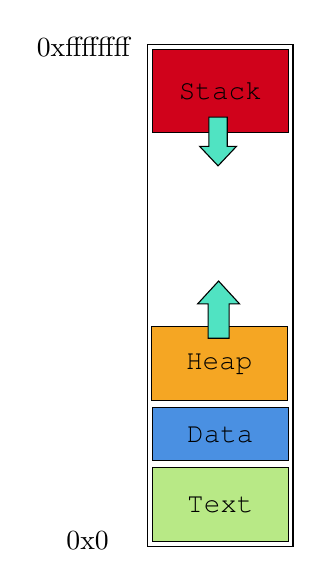
\begin{tikzpicture}[x=0.75pt,y=0.75pt,yscale=-1,xscale=1]
%uncomment if require: \path (0,300); %set diagram left start at 0, and has height of 300

%Shape: Rectangle [id:dp1982436807499255] 
\draw   (330,23) -- (400,23) -- (400,265) -- (330,265) -- cycle ;
%Shape: Rectangle [id:dp02798297576071851] 
\draw  [fill={rgb, 255:red, 184; green, 233; blue, 134 }  ,fill opacity=1 ] (332.25,227) -- (397.75,227) -- (397.75,262.5) -- (332.25,262.5) -- cycle ;
%Shape: Rectangle [id:dp8690208046922276] 
\draw  [fill={rgb, 255:red, 74; green, 144; blue, 226 }  ,fill opacity=1 ] (332.25,197.83) -- (397.75,197.83) -- (397.75,223.33) -- (332.25,223.33) -- cycle ;
%Shape: Rectangle [id:dp6529311675516911] 
\draw  [fill={rgb, 255:red, 245; green, 166; blue, 35 }  ,fill opacity=1 ] (331.75,158.83) -- (397.25,158.83) -- (397.25,194.58) -- (331.75,194.58) -- cycle ;
%Up Arrow [id:dp9371264302671377] 
\draw  [fill={rgb, 255:red, 80; green, 227; blue, 194 }  ,fill opacity=1 ] (354,148.03) -- (364.13,137) -- (374.25,148.03) -- (369.19,148.03) -- (369.19,164.58) -- (359.06,164.58) -- (359.06,148.03) -- cycle ;
%Shape: Rectangle [id:dp8515554275840291] 
\draw  [fill={rgb, 255:red, 208; green, 2; blue, 27 }  ,fill opacity=1 ] (332.25,25.5) -- (397.75,25.5) -- (397.75,65.5) -- (332.25,65.5) -- cycle ;
%Down Arrow [id:dp38470823955499234] 
\draw  [fill={rgb, 255:red, 80; green, 227; blue, 194 }  ,fill opacity=1 ] (355,72.1) -- (359.44,72.1) -- (359.44,58) -- (368.31,58) -- (368.31,72.1) -- (372.75,72.1) -- (363.88,81.5) -- cycle ;

% Text Node
\draw (365,211.25) node   [align=left] {{\fontfamily{pcr}\selectfont Data}};
% Text Node
\draw (365,244.75) node   [align=left] {{\fontfamily{pcr}\selectfont Text}};
% Text Node
\draw (364.5,176.71) node   [align=left] {{\fontfamily{pcr}\selectfont Heap}};
% Text Node
\draw (365,45.5) node   [align=left] {{\fontfamily{pcr}\selectfont Stack}};
% Text Node
\draw (299,24) node   [align=left] {0xffffffff};
% Text Node
\draw (301,262) node   [align=left] {0x0};



\end{tikzpicture}

\end{center}


Your program is allocated a certain block of memory- within it are the following 4 components. Keep in mind that this too, is an abstraction. You can further explore how programs are represented in memory in classes like CMSC411, but this is just about as far as we'll go in 216.

\begin{itemize}
	\item \textbf{Text} is where the code for your program goes. It's really not much more complex than that.
	\item \textbf{Data} is where global variables and variables that are static belong.
	\item \textbf{Heap} is where dynamically allocated memory lives. In Java, this stuff was managed for you. In C, you will have to manage it yourself, allocating memory and effectively increasing the size of the heap if you need more space while your program is running, and deallocating (freeing) memory to decrease the size of the heap. More on this when we discuss dynamically allocated memory.
	\item \textbf{Stack} is where local variables and function parameters live. It grows downwards (eventually meeting the heap and causing a stackoverflow) as functions are called. If you'll think back to 'stack frames' from recursion in CMSC132, this is the exact same concept.
\end{itemize}

\subsection{Storage}

There are two types of ways variables are stored in C- automatic and static. This basically goes hand-in-hand with block scopes and file scopes, but the important takeaways are these. First of all, in the example below, after the function \texttt{foo} is called, the variable \texttt{n} is thrown away.

{\centering
\begin{lstlisting}[language=C]
int foo(int k) {
	int n = 216;
	return n;
}
\end{lstlisting}
}

In that regard, the variable \texttt{n} has automatic storage. If a variable has static storage, it basically exists throughout the duration of your program's running time. Such variables are initialized only once.\newline

An important note: \texttt{static} in C does not mean the same thing as it does in Java. Here are the two main things that I think are worth remembering about static variables in C:

\begin{itemize}
	\item Static variables need not necessarily be initialized. If you don't bother initializing a static variable (you still have to declare it- this is not Python, language of the heathen) it will automatically initialize to zero.
	\item Static variables retain their values between function invocations. In other words, they are not stored using automatic storage.
\end{itemize}

{\centering
\begin{lstlisting}[language=C]
// example from Nelson Padua-Perez

void compute_static(int x) {                                                    
   static int value = 100; /* What would happen if we don't initialize it? */         
                                                                                
   printf("(static) x: %d, value: %d, sum: %d \n", x, value, value + x);        
                                                                                
   ++value;                                                                     
} 
\end{lstlisting}
}

In the example above, if you called \texttt{compute\_static} twice, then your output would be \texttt{(static) x: 1, value: 100, sum: 101} and \texttt{(static) x: 1, value: 101, sum: 102}, as 'value' would retain its data between function calls.

\subsection{Linkage}

Linkage is essentially the science behind having C code spread across multiple files and making sure it all compiles and works properly.\newline

We want to sometimes split code between multiple files for organizational purposes. Currently, the projects you're working on are small, but in order to make your programs versatile, modular and better organized, it's a great idea to split code between files.\newline

When you attempt this, there may be issues that follow. For example, you may encounter a situation where you want to name a function \texttt{print\_sum()} in two files. How would we deal with such a duplicate?\newline

Problems of this sort can be solved by adjusting the \textbf{linkage} of these functions.\newline

For actual code examples, please check the linkage-examples in the 216public directory. They're extremely thorough. My goal here is to provide a quick few tips on what I think are the most important parts.\newline

Essentially, there are three types of linkage that you should remember to guide you through writing code in multiple C files.

\begin{itemize}
	\item \textbf{\texttt{None}} $\rightarrow$ No linkage. This is how you usually declare your variables, and as you'd expect, doesn't do anything special in regards to linkage. Think of it this way: A variable with no linkage belongs to a single function, and cannot be shared. In other words, there is \textit{only one copy per declaration}.
	\item \textbf{\texttt{Internal}} $\rightarrow$ Internal linkage is just a fancy way of saying you're using the \textbf{\texttt{static}} keyword. All declarations of a single identifier in file refer to the same thing. In other words, there is \textit{only one copy per file}.
	\item \textbf{\texttt{External}} $\rightarrow$ External linkage is signified by the \texttt{extern} identifier, and it basically means that a name can only refer to a single entity in your entire program. In other words, there is \textit{only one copy per program}.
\end{itemize}

\subsection{Enumerated Types}

Enumerated Types, or enums, in C are pretty useful, and quite comparable to their equivalents in Java. The best way to understand enums (in my opinion) is to think of examples. Some good ones are an enum for the days of the week (Monday, Tuesday, etc.), seasons (Summer, Spring, Fall, Winter), or even suits in a deck of cards (Spades, Clubs, Hearts, Diamonds). Below is an example of the latter.

{\centering
\begin{lstlisting}[language=C]
// example from Nelson Padua-Perez
#include <stdio.h>
int main() {
	enum Suit {SPADES, HEARTS,DIAMONDS = 42, CLUBS};
	enum Suit suit1, suit2;
	suit1 = SPADES;
	suit2 = CLUBS;
	if (suit1 < suit2) printf("Spades are first.\n");
	else printf("Clubs are first.\n");
	printf("Spades = %d, Clubs = %d\n",suit1, suit2);
	return 0;
}
\end{lstlisting}
}

The functionality here is pretty basic, but one thing that I think is worth remembering (and quite nifty if you can use it well) is that enum representations are based in integers. This means that, for example, you can get away with adding the month enum for January (0) and the month enum for February (1) and end up with February (1).\newline

Again, the code above is a great example of how you can leverage the integer-like characteristics of enums.

\subsection{Implicit Type Conversion and Casting in C}

Switching between data types is pretty similar to how it was in Java, but here's a quick review of the stuff that matters. As you write your projects, you'll realize these things, but it's important to remember when it's a good idea to cast and when it isn't. Here are some general tips for you.\newline

\begin{itemize}
	\item \texttt There are a few ways to represent numbers in C. For relatively small numbers, \texttt{short}s are the way to go. If you want to represent a number that's a little bigger, use an \texttt{int}. The difference between these two on the systems that we'll be working with is that \texttt{int}s are twice the size of \texttt{short}s. (4 bytes vs. 2 bytes) If you want to represent a decimal number, You'll probably just want to use a \texttt{float}.
	\item In my opinion, most projects that we'll deal with here can be accomplished perfectly well with just \texttt{int}s and \texttt{float}s.
		\item We can also cast in C, and it works almost the same was as it did in Java. Just remember, in Java we had the concept of wrapper classes that allowed us to do fancy things with certain data types. In C, we don't enjoy that luxury, so we are restricted to just basic data type casting. Below is an example.
	
	
	{\centering
\begin{lstlisting}[language=C]
// example from Nelson Padua-Perez

#include <stdio.h>                                                                    
                                                                                      
int main() {                                                                          
   float x = 2.98;
   int y = (int)x;
}
\end{lstlisting}
}

\item That works exactly as you think it does. It converts 2.98 to 2 as it would in Java. Remember, don't overthink it, and don't try to call any wrapper class methods that you remember from Java. As long as you keep that in mind, you should be good to convert between data types in C.
\end{itemize}

	{\centering
\begin{lstlisting}[language=C]
// example from Nelson Padua-Perez

#include <stdio.h>                                                                    
                                                                                      
int main() {                                                                          
   int x = 2000000000;                                                                
   long result_long;                                                                  
                                                                                      
   printf("Value of x: %d\n", x);                                                     
   printf("Multiplying by 3 (with %%d format): %d\n", 2000000000 * 3);                
   printf("Multiplying by 3 (with %%ld format): %ld\n", 2000000000 * 3);              
   printf("Multiplying by 3L (with %%d format): %d\n", 2000000000 * 3L);              
   printf("Multiplying by 3L (with %%ld format): %ld\n", 2000000000 * 3L);            
                                                                                      
   result_long = 2000000000 * 3;  /* Does it solve the problem? */                    
   printf("Storing result in long type variable: %ld\n", result_long);                
                                                                                      
   return 0;                                                                          
}
\end{lstlisting}
}

The above example from Nelson isn't that basic, but I feel like it gives you a good insight into how type conversion can find use. Give that example a try to see a cool application of using multiple data types to handle larger values.

\section{Week 4}

This week we cover pointers, a few functions in C that you may find useful, and GDB in emacs. The main focus of these notes will be pointers, and chances are that you've seen a lot of this stuff in lecture as well. Make sure to take some time to try out the examples that we've got for you so you understand the basics of how pointers work, as they're a fundamental part of C.

\subsection{Pointers \& Memory Maps}

Let's go over pointers in C. You may have already covered this subject in lecture, but I'd like to point out some of the nuances that helped me understand pointers when I was taking 216. \newline

First of all, take note that pointers are just another type of variable. Just like you have \texttt{int}s and \texttt{char}s in C, which take up a certain amount of space and store a certain type of data, a \textbf{pointer} is a data type that stores an \textbf{address}. \newline

There are a bunch of ways to think of pointers, but I think the easiest way to understand them is to use memory maps. Think of them as as a tool to help us better understand how pointers work- they are essentially just visual representations of memory in C. \newline

I think that pointers and memory maps go hand in hand in 216, so I'll include some examples (some of my own, plus the examples we go over in discussion) that I think will help you become proficient with both pointers and memory maps. \newline

As a side note, you can take a look at Nelson's sample memory map online if you need some extra guidance. (This should have been covered in discussion). \newline

\texttt{\href{http://www.cs.umd.edu/~nelson/classes/resources/MemoryMapExample.pdf}{http://www.cs.umd.edu/~nelson/classes/resources/MemoryMapExample.pdf}}




\subsection{Example - Integer \& Integer Pointer\newline} 


{
\centering



\tikzset{every picture/.style={line width=0.75pt}} %set default line width to 0.75pt        

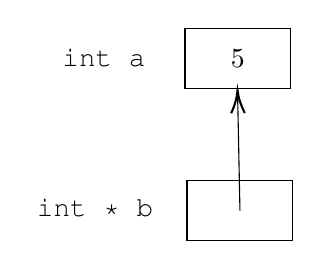
\begin{tikzpicture}[x=0.75pt,y=0.75pt,yscale=-1,xscale=1]
%uncomment if require: \path (0,300); %set diagram left start at 0, and has height of 300

%Shape: Rectangle [id:dp058944761853589434] 
\draw   (369,30) -- (420,30) -- (420,59.14) -- (369,59.14) -- cycle ;
%Shape: Rectangle [id:dp8289049315294679] 
\draw   (370,103.33) -- (421,103.33) -- (421,132.48) -- (370,132.48) -- cycle ;
%Straight Lines [id:da15432785379816327] 
\draw    (395.5,117.9) -- (394.37,62) ;
\draw [shift={(394.33,60)}, rotate = 448.85] [color={rgb, 255:red, 0; green, 0; blue, 0 }  ][line width=0.75]    (10.93,-3.29) .. controls (6.95,-1.4) and (3.31,-0.3) .. (0,0) .. controls (3.31,0.3) and (6.95,1.4) .. (10.93,3.29)   ;

% Text Node
\draw (330,44) node   [align=left] {{\fontfamily{pcr}\selectfont int a}};
% Text Node
\draw (394.5,44.57) node   [align=left] {5};
% Text Node
\draw (325.67,116.33) node   [align=left] {{\fontfamily{pcr}\selectfont int * b}};



\end{tikzpicture}

	
\begin{lstlisting}[language=C]
// example from Nelson Padua-Perez

#include <stdio.h>                                                                    
                                                                                      
int main() {                                                                          

	int a = 5;

	int * b = &a;   
	
	return 1;
}
\end{lstlisting}


}

This is about as simple as we can get with pointers. There are a variety of types of pointers that exist (one for each data type in C), but just remember that they're essentially just variables that store addresses.\newline

In this example, we can see that \texttt{a} is an integer, and \texttt{b} is an integer pointer. Although I've drawn an arrow from the inside of \texttt{b}'s box to \texttt{a}'s box, don't let that confuse you. \newline

Think of it like this- \texttt{a} \textbf{contains} the integer value 5. \texttt{b} \textbf{contains} the address of \texttt{a}. By convention in C, we say that \texttt{b} points to \texttt{a}. We just show this by drawing an arrow that starts in \texttt{b}'s box and points to \texttt{a}.

\subsection{Example - Multiple Pointer Types\newline}

{
\centering




\tikzset{every picture/.style={line width=0.75pt}} %set default line width to 0.75pt        

\begin{tikzpicture}[x=0.75pt,y=0.75pt,yscale=-1,xscale=1]
%uncomment if require: \path (0,300); %set diagram left start at 0, and has height of 300

%Shape: Rectangle [id:dp058944761853589434] 
\draw   (353,164) -- (404,164) -- (404,193.14) -- (353,193.14) -- cycle ;
%Shape: Rectangle [id:dp8289049315294679] 
\draw   (354,237.33) -- (405,237.33) -- (405,266.48) -- (354,266.48) -- cycle ;
%Straight Lines [id:da15432785379816327] 
\draw    (379.5,251.9) -- (378.37,196) ;
\draw [shift={(378.33,194)}, rotate = 448.85] [color={rgb, 255:red, 0; green, 0; blue, 0 }  ][line width=0.75]    (10.93,-3.29) .. controls (6.95,-1.4) and (3.31,-0.3) .. (0,0) .. controls (3.31,0.3) and (6.95,1.4) .. (10.93,3.29)   ;
%Shape: Rectangle [id:dp0020066675833932957] 
\draw   (223.67,28.67) -- (274.67,28.67) -- (274.67,57.81) -- (223.67,57.81) -- cycle ;
%Shape: Rectangle [id:dp16429220233511355] 
\draw   (224.67,102) -- (275.67,102) -- (275.67,131.14) -- (224.67,131.14) -- cycle ;
%Straight Lines [id:da051837340435018975] 
\draw    (250.17,116.57) -- (249.04,60.67) ;
\draw [shift={(249,58.67)}, rotate = 448.85] [color={rgb, 255:red, 0; green, 0; blue, 0 }  ][line width=0.75]    (10.93,-3.29) .. controls (6.95,-1.4) and (3.31,-0.3) .. (0,0) .. controls (3.31,0.3) and (6.95,1.4) .. (10.93,3.29)   ;
%Shape: Rectangle [id:dp1385770633532739] 
\draw   (465.67,28.67) -- (516.67,28.67) -- (516.67,57.81) -- (465.67,57.81) -- cycle ;
%Shape: Rectangle [id:dp03270745379570461] 
\draw   (467.33,105.33) -- (518.33,105.33) -- (518.33,134.48) -- (467.33,134.48) -- cycle ;
%Straight Lines [id:da3069083126116453] 
\draw    (492.17,116.57) -- (491.04,60.67) ;
\draw [shift={(491,58.67)}, rotate = 448.85] [color={rgb, 255:red, 0; green, 0; blue, 0 }  ][line width=0.75]    (10.93,-3.29) .. controls (6.95,-1.4) and (3.31,-0.3) .. (0,0) .. controls (3.31,0.3) and (6.95,1.4) .. (10.93,3.29)   ;

% Text Node
\draw (284.67,177.33) node   [align=left] {{\fontfamily{pcr}\selectfont double my\_double}};
% Text Node
\draw (378.5,178.57) node   [align=left] {9.0};
% Text Node
\draw (272.33,251.67) node   [align=left] {{\fontfamily{pcr}\selectfont double * double\_ptr}};
% Text Node
\draw (159.33,44) node   [align=left] {{\fontfamily{pcr}\selectfont int my\_integer}};
% Text Node
\draw (249.17,43.24) node   [align=left] {6};
% Text Node
\draw (151,113.67) node   [align=left] {{\fontfamily{pcr}\selectfont int * integer\_ptr}};
% Text Node
\draw (399.33,44) node   [align=left] {{\fontfamily{pcr}\selectfont char my\_char}};
% Text Node
\draw (491.17,43.24) node   [align=left] {e};
% Text Node
\draw (395,118.33) node   [align=left] {{\fontfamily{pcr}\selectfont char * char\_ptr}};


\end{tikzpicture}


	
\begin{lstlisting}[language=C]
// example from Nelson Padua-Perez

#include <stdio.h>                                                                    
                                                                                      
int main() {                                                                          

	int my\_integer = 6;
	double my\_double = 9.0;
	char my\_char = 'e';
	
	int * int\_ptr = &my\_integer;
	double * double\_ptr = &my\_double;
	char * char\_ptr = &my\_char;
	
}
\end{lstlisting}


}

Here's a similar case to up above, but I just wanted to demonstrate that there are different types of pointers. Now, keep in mind that all of these pointers essentially hold addresses, and it's not like the address of a double looks much different from the address of a character or the address of an integer.\newline

If you're wondering why C is so specific and asks you to define the type of pointer, the answer lies in how we will treat the data that's within the pointer. Sure, it may be that all pointers hold addresses, but what happens if we try to add the contents of \texttt{double\_ptr} and \texttt{integer\_ptr}? If C only had one pointer type and we tried to add the contents of those two pointers together, there would be no way of knowing that we made a mistake until runtime. In that sense, C maintains different types of pointers to ensure type compatibility. The same address could be given by the C memory manager to an integer pointer or a double pointer, but in order to make sure that you're treating whatever is stored at that address in a type-compatible way, C makes sure to note the type of what you're pointing to.


\subsection{Example - Pointer To a String (Char Array) \newline}

{
\centering






\tikzset{every picture/.style={line width=0.75pt}} %set default line width to 0.75pt        

\begin{tikzpicture}[x=0.75pt,y=0.75pt,yscale=-1,xscale=1]
%uncomment if require: \path (0,300); %set diagram left start at 0, and has height of 300

%Shape: Rectangle [id:dp16429220233511355] 
\draw   (245.67,207) -- (296.67,207) -- (296.67,236.14) -- (245.67,236.14) -- cycle ;
%Straight Lines [id:da051837340435018975] 
\draw    (271.17,221.57) -- (271.98,148.5) ;
\draw [shift={(272,146.5)}, rotate = 450.64] [color={rgb, 255:red, 0; green, 0; blue, 0 }  ][line width=0.75]    (10.93,-3.29) .. controls (6.95,-1.4) and (3.31,-0.3) .. (0,0) .. controls (3.31,0.3) and (6.95,1.4) .. (10.93,3.29)   ;
%Shape: Rectangle [id:dp8412783566407918] 
\draw   (243.67,117) -- (294.67,117) -- (294.67,146.14) -- (243.67,146.14) -- cycle ;
%Shape: Rectangle [id:dp7327342661859714] 
\draw   (294.67,117) -- (345.67,117) -- (345.67,146.14) -- (294.67,146.14) -- cycle ;
%Shape: Rectangle [id:dp03554725186896712] 
\draw   (345.67,117) -- (396.67,117) -- (396.67,146.14) -- (345.67,146.14) -- cycle ;
%Shape: Rectangle [id:dp5893017620753757] 
\draw   (396.67,117) -- (447.67,117) -- (447.67,146.14) -- (396.67,146.14) -- cycle ;
%Shape: Rectangle [id:dp8682717330515748] 
\draw   (447.67,117) -- (498.67,117) -- (498.67,146.14) -- (447.67,146.14) -- cycle ;

% Text Node
\draw (169,217.67) node   [align=left] {{\fontfamily{pcr}\selectfont char[5] my\_string}};
% Text Node
\draw (269.17,131.57) node   [align=left] {\textbackslash 0};
% Text Node
\draw (320.17,131.57) node   [align=left] {\textbackslash 0};
% Text Node
\draw (371.17,131.57) node   [align=left] {\textbackslash 0};
% Text Node
\draw (422.17,131.57) node   [align=left] {\textbackslash 0};
% Text Node
\draw (473.17,131.57) node   [align=left] {\textbackslash 0};


\end{tikzpicture}



	
\begin{lstlisting}[language=C]
// example from Nelson Padua-Perez

#include <stdio.h>                                                                    
                                                                                      
int main() {                                                                          

	char my_string[5];
	
}
\end{lstlisting}


}

Finally, here's a look at how we would store a string. I picked a string because it's essentially an array of characters, so we get to see how both are represented in memory maps. \newline

Here, don't let the notation confuse you. Although I've declared the string \texttt{my\_string} in special notation, it's still essentially a pointer to a character. In this case, \texttt{my\_string} is a pointer to the first of 5 characters that C has allocated as \texttt{NULL} for us. I've taken the liberty to fill the allocated blocks in as null bytes. 

\subsection{Lab Examples}

I'll also go over the examples that we went over in lab, but a little less in-depth, as they're usually a bunch of concepts put together. We'll focus on what I think are the important portions of each example.

\subsection{Example from Lab - ptr\_review.c}

Here, we'll talk a little bit about\texttt{ptr\_review.c} \newline (This file can be found at \texttt{~/216public/labs/Week4/lab1}) \newline

This is just going over the basics of pointers, and it has a few functions that demonstrate a few things, but I'd just like to go over a few of the questions posed in the actual file.

{
\centering
\begin{lstlisting}[language=C]
// example from Nelson Padua-Perez

int main(void) {   /* notice use of void in main */                                   
   float *p, *m;   /* have garbage value */                                           
   float pressure; /* has garbage value */                                            
   int area = 10;                                                                     
   int a[3] = {777, 888};  /* missing value? */                                       
                                                                                      
   p = &pressure;  /* & returns address */                                            
   m = p;          /* both m and p point to the same entity */                        
   printf("Value1 %.2f\n", *m); /* are we ever getting a segmentation fault?*/
   
   ...
	
   return 0;
   
}

\end{lstlisting}
}

\begin{itemize}
	\item Using the keyword \texttt{void} in main essentially means that your program will be taking no arguments. That's the long and short of it.
	\item When we define \texttt{p} and \texttt{m} as pointers and don't assign anything to them, they essentially contain garbage values. If you want a visual representation of that, just imagine two pointer variables with arrows pointing into the unknown. We don't know what they're pointing to, nor do we want to find out.
	\item It's the same deal if we define a float without assigning it a value- it contains a garbage value.
	\item When they set \texttt{m} equal to \texttt{p}, they're making it so both pointers are pointing to the same variable. If that confuses you, think of it the other way- pointers contain addresses, and it just so happens that after executing \texttt{m = p;}, both \texttt{m} and \texttt{p} contain the same addresses.
\end{itemize}

{
\centering


\tikzset{every picture/.style={line width=0.75pt}} %set default line width to 0.75pt        

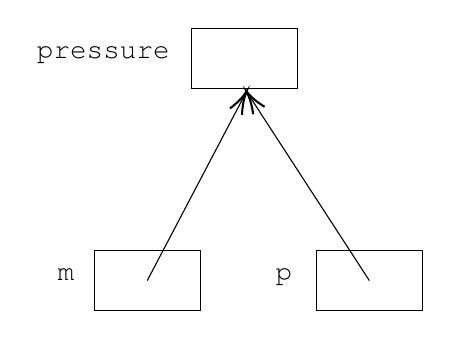
\begin{tikzpicture}[x=0.75pt,y=0.75pt,yscale=-1,xscale=1]
%uncomment if require: \path (0,300); %set diagram left start at 0, and has height of 300

%Shape: Rectangle [id:dp16429220233511355] 
\draw   (245.67,207) -- (296.67,207) -- (296.67,236.14) -- (245.67,236.14) -- cycle ;
%Straight Lines [id:da051837340435018975] 
\draw    (271.17,221.57) -- (318.07,132.27) ;
\draw [shift={(319,130.5)}, rotate = 477.71] [color={rgb, 255:red, 0; green, 0; blue, 0 }  ][line width=0.75]    (10.93,-3.29) .. controls (6.95,-1.4) and (3.31,-0.3) .. (0,0) .. controls (3.31,0.3) and (6.95,1.4) .. (10.93,3.29)   ;
%Shape: Rectangle [id:dp5176612453446056] 
\draw   (352.67,207) -- (403.67,207) -- (403.67,236.14) -- (352.67,236.14) -- cycle ;
%Straight Lines [id:da9913485463278986] 
\draw    (378.17,221.57) -- (320.09,132.18) ;
\draw [shift={(319,130.5)}, rotate = 416.99] [color={rgb, 255:red, 0; green, 0; blue, 0 }  ][line width=0.75]    (10.93,-3.29) .. controls (6.95,-1.4) and (3.31,-0.3) .. (0,0) .. controls (3.31,0.3) and (6.95,1.4) .. (10.93,3.29)   ;
%Shape: Rectangle [id:dp7874256794735744] 
\draw   (292.67,100) -- (343.67,100) -- (343.67,129.14) -- (292.67,129.14) -- cycle ;

% Text Node
\draw (232,218.67) node   [align=left] {{\fontfamily{pcr}\selectfont m}};
% Text Node
\draw (337,219.67) node   [align=left] {{\fontfamily{pcr}\selectfont p}};
% Text Node
\draw (250,112.67) node   [align=left] {{\fontfamily{pcr}\selectfont pressure}};


\end{tikzpicture}

}

\begin{itemize}
	\item Finally, when it asks if we are ever getting a segfault, the short answer is \textbf{maybe}. In C, dereferencing a pointer that we have not yet initialized is considered \textbf{undefined behavior}. It could provide us with garbage data, give us a segfault because we tried to access corrupted data, or give us a segfault because we tried to access data locked off by the system. We don't really know what will happen in this case, so we're calling it undefined behavior. In grace, variables that aren't initialized are given a value of 0 or NULL, so we won't see this effect here. However, running in any other C environment will yield undefined behavior.
\end{itemize}

\subsection{Example from Lab - ptr\_add\_sub\_overview.c}

Here, we'll talk a little bit about \texttt{ptr\_add\_sub\_overview.c} \newline (This file can be found at\texttt{~/216public/labs/Week4/lab1}) \newline

This example is all about pointer arithmetic, and it relies on the fact that you understand that arrays are stored in contiguous memory. Let's think about the following example. If you had an array that was represented in C memory like this:\newline\newline

{
\centering




\tikzset{every picture/.style={line width=0.75pt}} %set default line width to 0.75pt        

\begin{tikzpicture}[x=0.75pt,y=0.75pt,yscale=-1,xscale=1]
%uncomment if require: \path (0,300); %set diagram left start at 0, and has height of 300

%Shape: Rectangle [id:dp5176612453446056] 
\draw   (228.67,212) -- (279.67,212) -- (279.67,241.14) -- (228.67,241.14) -- cycle ;
%Straight Lines [id:da9913485463278986] 
\draw    (254.17,226.57) -- (258.9,132.5) ;
\draw [shift={(259,130.5)}, rotate = 452.88] [color={rgb, 255:red, 0; green, 0; blue, 0 }  ][line width=0.75]    (10.93,-3.29) .. controls (6.95,-1.4) and (3.31,-0.3) .. (0,0) .. controls (3.31,0.3) and (6.95,1.4) .. (10.93,3.29)   ;
%Shape: Rectangle [id:dp7874256794735744] 
\draw   (234.67,99) -- (285.67,99) -- (285.67,128.14) -- (234.67,128.14) -- cycle ;
%Shape: Rectangle [id:dp04481985338500627] 
\draw   (285.67,99) -- (336.67,99) -- (336.67,128.14) -- (285.67,128.14) -- cycle ;
%Shape: Rectangle [id:dp7253813806088456] 
\draw   (336.67,99) -- (387.67,99) -- (387.67,128.14) -- (336.67,128.14) -- cycle ;
%Shape: Rectangle [id:dp7617124294428573] 
\draw   (387.67,99) -- (438.67,99) -- (438.67,128.14) -- (387.67,128.14) -- cycle ;
%Shape: Rectangle [id:dp12383450763178705] 
\draw   (438.67,99) -- (489.67,99) -- (489.67,128.14) -- (438.67,128.14) -- cycle ;

% Text Node
\draw (213,224.67) node   [align=left] {{\fontfamily{pcr}\selectfont p}};
% Text Node
\draw (260.17,113.57) node   [align=left] {1};
% Text Node
\draw (311.17,113.57) node   [align=left] {6};
% Text Node
\draw (362.17,113.57) node   [align=left] {6};
% Text Node
\draw (413.17,113.57) node   [align=left] {1};
% Text Node
\draw (464.17,113.57) node   [align=left] {2};


\end{tikzpicture}


}


In this case, since arrays are stored in contiguous memory, so essentially what we are claiming with pointer arithmetic is that, if we dereference \texttt{p} now, we will get the number 1. If we \textbf{add} 1 to p (the actual pointer) and then dereference it, we will get the number 6. The file explores similar examples. Here are some highlights.

\begin{itemize}
	\item Just like we discussed earlier, here's an application of simple pointer addition. As a reminder you can add numbers other than 1.
	\begin{lstlisting}[language=C]
// example from Nelson Padua-Perez

char name[MAX] = "The House is Blue";                                              
   char *p = name, *q;                                                                
   int i;                                                                             
                                                                                      
   /* You can add and subtract integer values from pointers.   */                     
   /* For example, if you add one to a pointer to a character  */                     
   /* array, the pointer will now be referring to the next     */                     
   /* character.  You can add any integer value (not just one) */                     
                                                                                      
   /* Printing the string using pointer arithmetic */                                 
   while (*p != '\0') {                                                               
      printf("%c", *p);                                                               
      p = p + 1;                                                                      
   }
   
}

\end{lstlisting}

	\item You can also take advantage of the fact that arrays are stored in contiguous memory by subtracting pointers to find 'distance' between them. Note that this only works with pointers of the same type.
	
\begin{lstlisting}[language=C]
// example from Nelson Padua-Perez

   /* You can tell how many elements are between two pointers */                      
   /* by subtracting pointers */                                                      
   p = name + 1;                                                                      
   q = &name[5];                                                                      
   printf("Elements #1: %ld\n", q - p);                                               
   printf("Elements #2: %ld\n", p - q);

\end{lstlisting}

\item Finally, you can leverage pointer arithmetic to help you index arrays as well. Here's an example of that below.


\begin{lstlisting}[language=C]
// example from Nelson Padua-Perez

   /* Indexing is a pointer operation */                                              
   printf("Indexing as pointer operation\n");                                         
   p = name;                                                                          
   for (i = 0; i < strlen(name); i++) {                                               
      printf("%c\n", p[i]);                                                           
   }

\end{lstlisting}

	
\end{itemize}

\subsection{Example from Lab - str\_review.c}

Here, we'll talk a little bit about\texttt{str\_review.c} \newline (This file can be found at \texttt{~/216public/labs/Week4/lab1}) \newline

This example is pretty light compared to the rest- and it is just a review of how strings are stored in C. The main overarching concept you need to understand here is two things:

\begin{itemize}
	\item Strings are not given an actual data type in C. They are simply arrays of characters with a small caveat.
	\item That being said, strings are always stored in a certain way. They are a character array terminated with a null byte. (No null byte at the end means you don't have a string- you have a regular old character array)
\end{itemize}

Take a look at my String example above for the memory map representation.

\subsection{Using getchar() and putchar()}

The two functions \texttt{getchar} and \texttt{putchar} are pretty curious, in that we have much more functional replacements for them- \texttt{scanf} and \texttt{printf}, respectively. However, learning these is a cool way to prep yourself for how basic I/O in assembly works, so I think that it's worth it to at least gloss over these for now. \newline

Let's look over the code provided for us in discussion and touch on the main points.

\begin{lstlisting}[language=C]
// example from Nelson Padua-Perez

#include <stdio.h>                                                                    
                                                                                      
#define MAX_LEN 80                                                                    
                                                                                      
int main() {                                                                          
   char value[MAX_LEN + 1];                                                           
   int letter; /* Why integer? */                                                     
                                                                                      
   printf("Enter a letter: ");                                                        
   scanf("%1s", value);                                                               
   printf("Value entered: \"%s\"\n", value);                                          
   getchar();   /* getchar() reads a single character; why we need it? */             
   printf("Enter a letter: ");                                                        
   letter = getchar();                                                                
   printf("Letter entered: ");                                                        
   putchar(letter);      /* putchar() prints a single character */                    
   printf("\n");                                                                      
                         /* try ungetc to put characters back */                      
                                                                                      
   return 0;                                                                          
}  
\end{lstlisting}

\begin{itemize}
	\item First of all, both \texttt{getchar} and \texttt{putchar} deal with integers, despite the fact that they are meant to take in/print characters. Don't let this confuse you, they're simply storing them by the ASCII value.
	\item Both of these get and print a single character, and in my opinion, there's no real reason to need them except in very special cases, but this is how I/O will be conducted in Assembly, so I think it's worth taking a look at this now.
	\item Your main takeaway from this should be that \texttt{getchar} and \texttt{putchar} are functions that we can use to do I/O in C, and even though they're a little more crude than we'd like for most applications, they still exist, and are helpful tools when we're trying to understand Assembly.
\end{itemize}

\section{Week 5}

\subsection{Grep - A 'CTRL-F' From the Command Line}

When working with the command line, we have the unique opportunity to see older versions of computer tools that we are accustomed to today. In modern environments, if you want to find something on a webpage, textbook, or even in your \texttt{.java} file in Eclipse, the first thing that probably comes to you head is the command '\texttt{CTRL + F}'. In a command line environment, the command that preceded this functionality is known as \texttt{grep}. 

\subsubsection{Why is it called that?}
The name of the command itself has an interesting origin. The most basic text editor on UNIX systems is regarded by many as \texttt{ed}, and on that text editor, one was able to globally search the file for a regular expression (which you'll learn morere about in CMSC330), then print what was found using the command '\texttt{g/re/p}'. This gave way to the name "grep".

\subsubsection{Why it's useful}

As you'd imagine, grep can be used to simply search the files we have for keywords. Let's take a look at some examples. You can follow along if you head over to \texttt{216public/labs/Week5/lab 1/grep\_example}.

Let's take a look at the text files that we will be searching through, as examples.

\begin{lstlisting}[language=C]
The college is in
the east coast.  
\end{lstlisting}
\begin{center}
\textbf{data.txt}
\end{center}


\begin{lstlisting}[language=C]
The project is about hashing,
files, structures,
pointers
and dynamic memory allocation (and more pointers).  
\end{lstlisting}
\begin{center}
\textbf{summary.txt}
\end{center}


These two files are in the same directory, and for the purpose of the examples I'll go over, let's assume that we're currently in the directory that contains both these files.\newline

\texttt{grep} works like this: you provide it a key phrase and a file location, and it'll take care of the rest. If you want more technical information on how grep commands should be structured, I encourage you to take a look at \texttt{man grep}. \newline

If you execute the command \texttt{grep college data.txt}, then grep will print out the line that it found your keyword on. (the output for that command will be \texttt{The college is in}.)\newline

Where \texttt{grep} really shines is when you want to mix in some of the cool UNIX keywords we've been learning. As a quick example, let's say you wanted to search for all the occurrences of 'is' in all the text files you had in the file. To do that, you'd simply execute the following command.\newline

\texttt{grep is *}\newline

That would yield the following:\newline

\texttt{data.txt:The college is in\newline
summary.txt:The project is about hashing,
}\newline

In a more practical example, let's think about how you could use this when writing your projects. Let's say you had a particularly tough project with 20 public tests. You're failing a bunch of them, but you suspect it's because the tests are calling a function you know you haven't implemented properly yet, named \texttt{get\_classroom\_number()}.\newline

Assuming that public test files are named as they usually are in this class, and that you're in your project directory, if you wanted to figure out which public tests were testing for the \texttt{get\_classroom\_number()} function, all you have to do is cook up a \texttt{grep} command to do that for you. Here's what we'd be looking at in this case:\newline

\texttt{grep get\_classroom\_number() public*}\newline

This would search for the keyword \texttt{get\_classroom\_number()} in every file that started with 'public', which is exactly what we want. (Remember your UNIX special characters!). Additionally, here's one extra little trick that might make grepping a little bit easier- if you want to see the line numbers that your searches actually appear on, go ahead and use the \texttt{-n} flag when you run grep. The previous example would then look like this:\newline

\texttt{grep -n get\_classroom\_number() public*}

\subsection{Memcpy, Memmove, and Memset}

In C, we sometimes want to simply just manipulate blocks of memory. Although we were previously able to do this with strings, we can also do this at a much less abstracted level, and just mess with the memory itself.\newline

I suggest that you follow along using the lab example named \texttt{mem\_cpy\_set.c} located at: \newline \texttt{216public/labs/Week5/lab 1}

\begin{itemize}
	\item \textbf{\texttt{void *memcpy(void *dest, const void *src, size\_t n)}} - memcpy is a function that simply copies memory from one block to another, and that's the gist of it. The two main uses we have for this are to (1) copy strings from one location to another (but for this case, you're probably better off using strcpy or strncpy) and (2) to copy structs from one location to another. As you can see, the function asks for an unsigned integer 'n', which we can usually mark off as the \texttt{sizeof(struct\_you\_want\_to\_copy)}.
	\item \textbf{\texttt{void *memmove(void *dest, const void *src, size\_t n)}} - This one is basically the same as memcpy, but you'll want to use this when the memory you need to copy \textbf{to} overlaps with the memory you want to copy \textbf{from}.
	\item \textbf{\texttt{void *memset(void *str, int c, size\_t n)}} - This is a pretty niche command, and the gist of it is this. It'll take the block of memory that you specify, and set it all to a certain value that you specify. I can see this being useful if you wanted to set all the values in a contiguous array to the number '1' as a default value, or something like that.\newline

\end{itemize}

As a final side note, you can get more information on all three of these functions by using \texttt{man}. However, you will need to provide the '3' flag when you invoke the man command, so your commands would look like the following.

\begin{itemize}
	\item \texttt{man 3 memcpy}
	\item \texttt{man 3 memset}
	\item \texttt{man 3 memmove}
\end{itemize}

\section{Week 6}

This week is a quiz week, so we held open office hours during discussion and answered specific questions. Honestly, for reviews for quizzes, I would highly recommend checking Piazza for the answers and clarifications that you're looking for. In this guide, since we really just went over specifics during discussion before the quiz, I'm going to skip over this and get straight to what we covered after the quiz.

\subsection{Preprocessor}

To follow along with these notes, I'd recommend taking a look at '\texttt{PreprocessorI.pdf (Lab)} from the Week 6 section on the 'Schedule' page of the course website.\newline

Here, we'll be talking a little bit about C's preprocessing and compiling. Preprocessing is essentially the stuff that C provides for your code right before it compiles, e.g. replacing macros with their appropriate text values.

\subsubsection{Compiling a C Program}

When you compile a C program, a few things happen behind the scenes. First, a source file (\texttt{.c}) is compiled into an object file (\texttt{.o}). Think of the object file as an intermediary step between a C file and an executable. An object file isn't necessarily an executable let, but it's about halfway there. This'll help us a lot more when we talk about \texttt{make}, but for now, that's all you really need to remember.\newline

After an object file is created, it can be compiled into an executable, which is usually done by the linker. Essentially, the linker just does some cleanup work with symbols that you've defined, global variables, and other data.\newline


{
\centering






\tikzset{every picture/.style={line width=0.75pt}} %set default line width to 0.75pt        

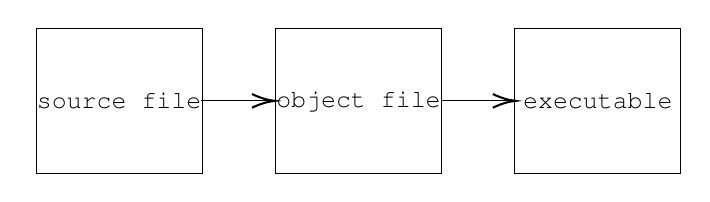
\begin{tikzpicture}[x=0.75pt,y=0.75pt,yscale=-1,xscale=1]
%uncomment if require: \path (0,300); %set diagram left start at 0, and has height of 300

%Flowchart: Process [id:dp9087722479160656] 
\draw   (100,59) -- (180,59) -- (180,129) -- (100,129) -- cycle ;
%Flowchart: Process [id:dp18707723736432025] 
\draw   (215.33,59) -- (295.33,59) -- (295.33,129) -- (215.33,129) -- cycle ;
%Flowchart: Process [id:dp26379991992077745] 
\draw   (330.67,59) -- (410.67,59) -- (410.67,129) -- (330.67,129) -- cycle ;
%Straight Lines [id:da45725440322215305] 
\draw    (179.67,94) -- (213,94) ;
\draw [shift={(215,94)}, rotate = 180] [color={rgb, 255:red, 0; green, 0; blue, 0 }  ][line width=0.75]    (10.93,-3.29) .. controls (6.95,-1.4) and (3.31,-0.3) .. (0,0) .. controls (3.31,0.3) and (6.95,1.4) .. (10.93,3.29)   ;
%Straight Lines [id:da739474493577637] 
\draw    (295.67,94) -- (329,94) ;
\draw [shift={(331,94)}, rotate = 180] [color={rgb, 255:red, 0; green, 0; blue, 0 }  ][line width=0.75]    (10.93,-3.29) .. controls (6.95,-1.4) and (3.31,-0.3) .. (0,0) .. controls (3.31,0.3) and (6.95,1.4) .. (10.93,3.29)   ;

% Text Node
\draw (140,94) node   [align=left] {{\fontfamily{pcr}\selectfont {\small source file}}};
% Text Node
\draw (255.33,94) node   [align=left] {{\fontfamily{pcr}\selectfont {\small object file}}};
% Text Node
\draw (370.67,94) node   [align=left] {{\small {\fontfamily{pcr}\selectfont executable}}};


\end{tikzpicture}



}

\subsubsection{Preproccessor Defined Symbols}

There are a few symbols that C will recognize and replace with text during preprocessing. For example, typing \texttt{\_\_DATE\_\_} in your C file will cause C to replace it with the date of compilation when you actually compile your program. Here's a list of these macros. (I've decided to exclude \texttt{\_\_STDC\_\_} only because we basically never see a use for it during 216.

\begin{itemize}
	\item \textbf{\texttt{\_\_FILE\_\_}} $\rightarrow$ filename of the source file that this macro is in.
	\item \textbf{\texttt{\_\_LINE\_\_}} $\rightarrow$ the line number that this macro is typed on. I've used this for debugging before- for example, let's say you're using a bunch of print statements throughout your code to see where it got to before a segfault. Instead of printing something like 'got here' for every statement, maybe write something where you \texttt{printf} something with \texttt{\_\_LINE\_\_} in it, then copy paste that statement into your code a bunch of times. It's a super easy way to see how far you get.
	\item \textbf{\texttt{\_\_DATE\_\_}} $\rightarrow$ the date of compilation. Not much to say here, it's more gimmicky than anything.
	\item \textbf{\texttt{\_\_TIME\_\_}} $\rightarrow$ same as above, except it's the time of compilation.
\end{itemize}

I would think of these like your \texttt{\#define} keywords. In this case, C is just looking for these particular strings, and replacing them with their corresponding replacements. These are useful mainly only for niche cases, like if you wanted your code to print out when it was compiled.\newline

Also, you've probably seen this a bunch by now, but \texttt{\#define} is basically just telling the C compiler to find all occurrences of one thing, and replace it with another thing. For example, doing something like \texttt{\#define MAX\_CHAR\_AMT 80} would cause the C compiler to find every occurrence of the string '\texttt{MAX\_CHAR\_AMT}' in your code and replace it with \texttt{80}. In that sense, the most prominent use for this in 216 is to define maximum size limits. If you need a reference, most projects will have these limits defined either in the base C files or the header files that they provide.

\subsubsection{Conditional Compilation}

Conditional compilation is an interesting topic, and I think the slides explain it pretty well. However, I think there are simpler examples than what's provided in the slides that'll help us understand it on a basic level.\newline

I suggest taking a look at \texttt{\href{https://www.programmingsimplified.com/c/tutorial/conditional-compilation}{https://www.programmingsimplified.com/c/tutorial/conditional-compilation}} for a really simple example that'll get you started.\newline

The main use of conditional compilation is basically that- if code should be written the same (i.e. the same C file) on two systems, but should be compiled differently based on other files that influence it or the system it's being compiled on, then conditional compilation is what you need. We don't see too much of this stuff in your projects, but it's good to know in case it pops up on an exam.

\subsubsection{File Inclusion}

File inclusion is sort of a self explanatory topic. Although we go over it formally in discussion and the preprocessor slides, I think the best way to understand this is to see real world examples. Luckily, you've done a few projects so far, and they're essentially working examples of how file inclusion should be done in C. For this topic, I invite you to take a look at your projects and see where header files are included, if there's ever multiple header files included, and, if you really want to explore, feel free to go back and mess with old projects. Change header files around, try to make a C file include multiple header files, change the order in which they're included, etc. You've been working with file inclusion this whole time, so feel free to experiment a bit with it and really get familiar. That, plus the theoretical background that the slides provide should be all you need.

\section{Week 7}

This week, we're going over new things after the Exam. We'll talk a little about Make, which allows us to easily compile our projects in C, Struct Abstraction, which is about as far as C goes in terms of emulating object oriented features, and dynamic memory allocation.

\subsection{Make}

To follow along with these notes, I'd recommend taking a look at '\texttt{Make.pdf (Lab)} from the Week 7 section on the 'Schedule' page of the course website.\newline

Before, if you wanted to compile a bunch of files at once, you'd just toss them all into one gcc command, like so:\newline

\texttt{gcc hashtable.c public01.c}\newline

Now this is fine, but as you can imagine, if you have a much larger C project with plenty of files (some depending on others, some not depending on others), you might run into some issues if you have to manually \texttt{gcc} everything each time you want to run your code. Luckily, C's got a solution for you!\newline

\subsubsection{Compiling into Object Code First}

Just a little note before we get into it- we've been skipping a step in terms of how code gets compiled. Just like I talked about above,  in the Preprocessor section, C gets compiled from source code to an object file to an executable, and so far, we've just been compiling straight from source code to executable. In order to fully understand \texttt{make}, we're going to want to note that we will now be compiling first into object files, then into source code.

\subsubsection{Dependencies}

First thing you need to know about \texttt{make}- it's all about dependencies. Let's say we had some C files, and for this example, let's go ahead and take a look at the example that they provide in the slides.\newline

{
\centering


\tikzset{every picture/.style={line width=0.75pt}} %set default line width to 0.75pt        

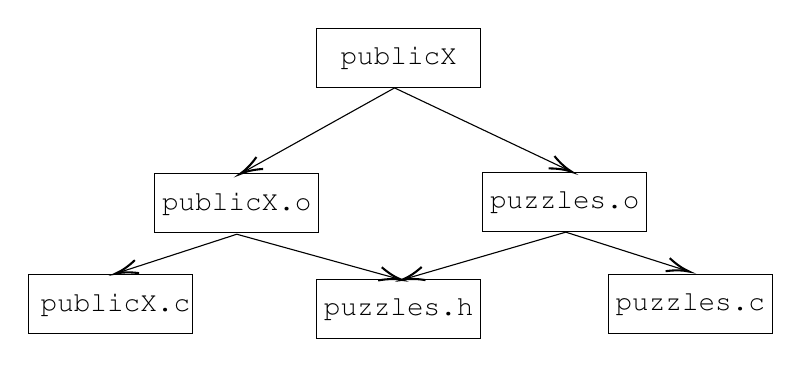
\begin{tikzpicture}[x=0.75pt,y=0.75pt,yscale=-1,xscale=1]
%uncomment if require: \path (0,300); %set diagram left start at 0, and has height of 300

%Shape: Rectangle [id:dp04584351351591953] 
\draw   (300.5,51) -- (379.5,51) -- (379.5,79.5) -- (300.5,79.5) -- cycle ;
%Shape: Rectangle [id:dp869537413731065] 
\draw   (222.5,121) -- (301.5,121) -- (301.5,149.5) -- (222.5,149.5) -- cycle ;
%Shape: Rectangle [id:dp09744507127214364] 
\draw   (380.5,120.5) -- (459.5,120.5) -- (459.5,149) -- (380.5,149) -- cycle ;
%Shape: Rectangle [id:dp6441175322103412] 
\draw   (300.5,172) -- (379.5,172) -- (379.5,200.5) -- (300.5,200.5) -- cycle ;
%Shape: Rectangle [id:dp970334445840234] 
\draw   (161.5,169.5) -- (240.5,169.5) -- (240.5,198) -- (161.5,198) -- cycle ;
%Shape: Rectangle [id:dp4273912861487811] 
\draw   (441,169.5) -- (520,169.5) -- (520,198) -- (441,198) -- cycle ;
%Straight Lines [id:da5700845683815001] 
\draw    (338,79.75) -- (265.25,120.28) ;
\draw [shift={(263.5,121.25)}, rotate = 330.88] [color={rgb, 255:red, 0; green, 0; blue, 0 }  ][line width=0.75]    (10.93,-3.29) .. controls (6.95,-1.4) and (3.31,-0.3) .. (0,0) .. controls (3.31,0.3) and (6.95,1.4) .. (10.93,3.29)   ;
%Straight Lines [id:da1587431355483161] 
\draw    (338,79.75) -- (421.69,119.39) ;
\draw [shift={(423.5,120.25)}, rotate = 205.35] [color={rgb, 255:red, 0; green, 0; blue, 0 }  ][line width=0.75]    (10.93,-3.29) .. controls (6.95,-1.4) and (3.31,-0.3) .. (0,0) .. controls (3.31,0.3) and (6.95,1.4) .. (10.93,3.29)   ;
%Straight Lines [id:da7368979653415088] 
\draw    (262,150.25) -- (205.4,168.63) ;
\draw [shift={(203.5,169.25)}, rotate = 342.01] [color={rgb, 255:red, 0; green, 0; blue, 0 }  ][line width=0.75]    (10.93,-3.29) .. controls (6.95,-1.4) and (3.31,-0.3) .. (0,0) .. controls (3.31,0.3) and (6.95,1.4) .. (10.93,3.29)   ;
%Straight Lines [id:da015222657466875456] 
\draw    (262,150.25) -- (339.57,171.72) ;
\draw [shift={(341.5,172.25)}, rotate = 195.47] [color={rgb, 255:red, 0; green, 0; blue, 0 }  ][line width=0.75]    (10.93,-3.29) .. controls (6.95,-1.4) and (3.31,-0.3) .. (0,0) .. controls (3.31,0.3) and (6.95,1.4) .. (10.93,3.29)   ;
%Straight Lines [id:da20417970212364012] 
\draw    (420.5,149.25) -- (343.42,171.69) ;
\draw [shift={(341.5,172.25)}, rotate = 343.77] [color={rgb, 255:red, 0; green, 0; blue, 0 }  ][line width=0.75]    (10.93,-3.29) .. controls (6.95,-1.4) and (3.31,-0.3) .. (0,0) .. controls (3.31,0.3) and (6.95,1.4) .. (10.93,3.29)   ;
%Straight Lines [id:da3319626117155393] 
\draw    (420.5,149.25) -- (478.09,167.64) ;
\draw [shift={(480,168.25)}, rotate = 197.71] [color={rgb, 255:red, 0; green, 0; blue, 0 }  ][line width=0.75]    (10.93,-3.29) .. controls (6.95,-1.4) and (3.31,-0.3) .. (0,0) .. controls (3.31,0.3) and (6.95,1.4) .. (10.93,3.29)   ;

% Text Node
\draw (340,65.25) node   [align=left] {{\fontfamily{pcr}\selectfont publicX}};
% Text Node
\draw (262,135.25) node   [align=left] {{\fontfamily{pcr}\selectfont publicX.o}};
% Text Node
\draw (420,134.75) node   [align=left] {{\fontfamily{pcr}\selectfont puzzles.o}};
% Text Node
\draw (340,186.25) node   [align=left] {{\fontfamily{pcr}\selectfont puzzles.h}};
% Text Node
\draw (480.5,183.75) node   [align=left] {{\fontfamily{pcr}\selectfont puzzles.c}};
% Text Node
\draw (203.5,184.25) node   [align=left] {{\fontfamily{pcr}\selectfont publicX.c}};


\end{tikzpicture}


}

\subsubsection{A Broad Overview of Public Tests with Make}

As you can see, we have a pretty solid dependency tree here. Main takeaways: C files (the source files) are generally at the bottom of the tree, and they (combined with H files) compile into O files. To reiterate, (C) source files combine with (H) header files as they're compiled, and they become (O) object files. These object files are then compiled into one big executable, so you can run it very easily. The reason I like this provided example so much is because it's very similar to the public tests that you're provided in your projects. You've got \texttt{puzzles.c}, which we can say is like the file that you'll usually fill out and write yourself. You've got \texttt{puzzles.h}, which we can assume is some file full of constants and function prototypes that was probably provided to you when you copied the project over from \texttt{216public}, and finally, you've got \texttt{publicX.c}, which is the public test you're trying to run. In this case, in order for \texttt{publicX} to be created, the \texttt{make} utility has to combine the data from \texttt{publicX.c}, \texttt{puzzles.h}, and \texttt{puzzles.c}.\newline

Let's go over the questions provided in the slides.\newline

\begin{itemize}
	\item \textbf{What needs to be compiled if \texttt{publicX.c} is changed?}\newline
		
		

\tikzset{every picture/.style={line width=0.75pt}} %set default line width to 0.75pt        

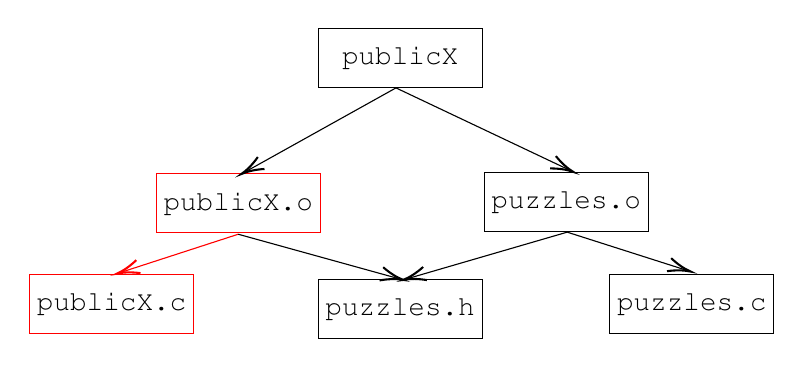
\begin{tikzpicture}[x=0.75pt,y=0.75pt,yscale=-1,xscale=1]
%uncomment if require: \path (0,300); %set diagram left start at 0, and has height of 300

%Shape: Rectangle [id:dp04584351351591953] 
\draw  [color={rgb, 255:red, 0; green, 0; blue, 0 }  ,draw opacity=1 ] (300.5,51) -- (379.5,51) -- (379.5,79.5) -- (300.5,79.5) -- cycle ;
%Shape: Rectangle [id:dp869537413731065] 
\draw  [color={rgb, 255:red, 255; green, 0; blue, 0 }  ,draw opacity=1 ] (222.5,121) -- (301.5,121) -- (301.5,149.5) -- (222.5,149.5) -- cycle ;
%Shape: Rectangle [id:dp09744507127214364] 
\draw   (380.5,120.5) -- (459.5,120.5) -- (459.5,149) -- (380.5,149) -- cycle ;
%Shape: Rectangle [id:dp6441175322103412] 
\draw   (300.5,172) -- (379.5,172) -- (379.5,200.5) -- (300.5,200.5) -- cycle ;
%Shape: Rectangle [id:dp970334445840234] 
\draw  [color={rgb, 255:red, 255; green, 0; blue, 0 }  ,draw opacity=1 ] (161.5,169.5) -- (240.5,169.5) -- (240.5,198) -- (161.5,198) -- cycle ;
%Shape: Rectangle [id:dp4273912861487811] 
\draw   (441,169.5) -- (520,169.5) -- (520,198) -- (441,198) -- cycle ;
%Straight Lines [id:da5700845683815001] 
\draw [color={rgb, 255:red, 0; green, 0; blue, 0 }  ,draw opacity=1 ]   (338,79.75) -- (265.25,120.28) ;
\draw [shift={(263.5,121.25)}, rotate = 330.88] [color={rgb, 255:red, 0; green, 0; blue, 0 }  ,draw opacity=1 ][line width=0.75]    (10.93,-3.29) .. controls (6.95,-1.4) and (3.31,-0.3) .. (0,0) .. controls (3.31,0.3) and (6.95,1.4) .. (10.93,3.29)   ;
%Straight Lines [id:da1587431355483161] 
\draw    (338,79.75) -- (421.69,119.39) ;
\draw [shift={(423.5,120.25)}, rotate = 205.35] [color={rgb, 255:red, 0; green, 0; blue, 0 }  ][line width=0.75]    (10.93,-3.29) .. controls (6.95,-1.4) and (3.31,-0.3) .. (0,0) .. controls (3.31,0.3) and (6.95,1.4) .. (10.93,3.29)   ;
%Straight Lines [id:da7368979653415088] 
\draw [color={rgb, 255:red, 255; green, 0; blue, 0 }  ,draw opacity=1 ]   (262,150.25) -- (205.4,168.63) ;
\draw [shift={(203.5,169.25)}, rotate = 342.01] [color={rgb, 255:red, 255; green, 0; blue, 0 }  ,draw opacity=1 ][line width=0.75]    (10.93,-3.29) .. controls (6.95,-1.4) and (3.31,-0.3) .. (0,0) .. controls (3.31,0.3) and (6.95,1.4) .. (10.93,3.29)   ;
%Straight Lines [id:da015222657466875456] 
\draw    (262,150.25) -- (339.57,171.72) ;
\draw [shift={(341.5,172.25)}, rotate = 195.47] [color={rgb, 255:red, 0; green, 0; blue, 0 }  ][line width=0.75]    (10.93,-3.29) .. controls (6.95,-1.4) and (3.31,-0.3) .. (0,0) .. controls (3.31,0.3) and (6.95,1.4) .. (10.93,3.29)   ;
%Straight Lines [id:da20417970212364012] 
\draw    (420.5,149.25) -- (343.42,171.69) ;
\draw [shift={(341.5,172.25)}, rotate = 343.77] [color={rgb, 255:red, 0; green, 0; blue, 0 }  ][line width=0.75]    (10.93,-3.29) .. controls (6.95,-1.4) and (3.31,-0.3) .. (0,0) .. controls (3.31,0.3) and (6.95,1.4) .. (10.93,3.29)   ;
%Straight Lines [id:da3319626117155393] 
\draw    (420.5,149.25) -- (478.09,167.64) ;
\draw [shift={(480,168.25)}, rotate = 197.71] [color={rgb, 255:red, 0; green, 0; blue, 0 }  ][line width=0.75]    (10.93,-3.29) .. controls (6.95,-1.4) and (3.31,-0.3) .. (0,0) .. controls (3.31,0.3) and (6.95,1.4) .. (10.93,3.29)   ;

% Text Node
\draw (340,65.25) node   [align=left] {{\fontfamily{pcr}\selectfont publicX}};
% Text Node
\draw (262,135.25) node   [align=left] {{\fontfamily{pcr}\selectfont publicX.o}};
% Text Node
\draw (420,134.75) node   [align=left] {{\fontfamily{pcr}\selectfont puzzles.o}};
% Text Node
\draw (340,186.25) node   [align=left] {{\fontfamily{pcr}\selectfont puzzles.h}};
% Text Node
\draw (480.5,183.75) node   [align=left] {{\fontfamily{pcr}\selectfont puzzles.c}};
% Text Node
\draw (201,183.75) node   [align=left] {{\fontfamily{pcr}\selectfont publicX.c}};


\end{tikzpicture}\newline

	Well, since we're changing the \texttt{.c} source file, we can safely assume that the object file that it will eventually become needs to be recompiled, so let's travel up one node on the dependency tree and mark that as 'need to be recompiled'. However, it doesn't stop there. \newline
	
	

\tikzset{every picture/.style={line width=0.75pt}} %set default line width to 0.75pt        

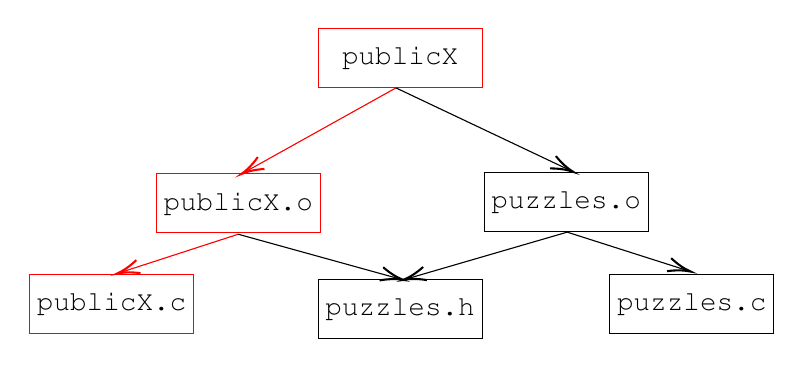
\begin{tikzpicture}[x=0.75pt,y=0.75pt,yscale=-1,xscale=1]
%uncomment if require: \path (0,300); %set diagram left start at 0, and has height of 300

%Shape: Rectangle [id:dp04584351351591953] 
\draw  [color={rgb, 255:red, 255; green, 0; blue, 0 }  ,draw opacity=1 ] (300.5,51) -- (379.5,51) -- (379.5,79.5) -- (300.5,79.5) -- cycle ;
%Shape: Rectangle [id:dp869537413731065] 
\draw  [color={rgb, 255:red, 255; green, 0; blue, 0 }  ,draw opacity=1 ] (222.5,121) -- (301.5,121) -- (301.5,149.5) -- (222.5,149.5) -- cycle ;
%Shape: Rectangle [id:dp09744507127214364] 
\draw   (380.5,120.5) -- (459.5,120.5) -- (459.5,149) -- (380.5,149) -- cycle ;
%Shape: Rectangle [id:dp6441175322103412] 
\draw   (300.5,172) -- (379.5,172) -- (379.5,200.5) -- (300.5,200.5) -- cycle ;
%Shape: Rectangle [id:dp970334445840234] 
\draw  [color={rgb, 255:red, 255; green, 0; blue, 0 }  ,draw opacity=1 ] (161.5,169.5) -- (240.5,169.5) -- (240.5,198) -- (161.5,198) -- cycle ;
%Shape: Rectangle [id:dp4273912861487811] 
\draw   (441,169.5) -- (520,169.5) -- (520,198) -- (441,198) -- cycle ;
%Straight Lines [id:da5700845683815001] 
\draw [color={rgb, 255:red, 255; green, 0; blue, 0 }  ,draw opacity=1 ]   (338,79.75) -- (265.25,120.28) ;
\draw [shift={(263.5,121.25)}, rotate = 330.88] [color={rgb, 255:red, 255; green, 0; blue, 0 }  ,draw opacity=1 ][line width=0.75]    (10.93,-3.29) .. controls (6.95,-1.4) and (3.31,-0.3) .. (0,0) .. controls (3.31,0.3) and (6.95,1.4) .. (10.93,3.29)   ;
%Straight Lines [id:da1587431355483161] 
\draw    (338,79.75) -- (421.69,119.39) ;
\draw [shift={(423.5,120.25)}, rotate = 205.35] [color={rgb, 255:red, 0; green, 0; blue, 0 }  ][line width=0.75]    (10.93,-3.29) .. controls (6.95,-1.4) and (3.31,-0.3) .. (0,0) .. controls (3.31,0.3) and (6.95,1.4) .. (10.93,3.29)   ;
%Straight Lines [id:da7368979653415088] 
\draw [color={rgb, 255:red, 255; green, 0; blue, 0 }  ,draw opacity=1 ]   (262,150.25) -- (205.4,168.63) ;
\draw [shift={(203.5,169.25)}, rotate = 342.01] [color={rgb, 255:red, 255; green, 0; blue, 0 }  ,draw opacity=1 ][line width=0.75]    (10.93,-3.29) .. controls (6.95,-1.4) and (3.31,-0.3) .. (0,0) .. controls (3.31,0.3) and (6.95,1.4) .. (10.93,3.29)   ;
%Straight Lines [id:da015222657466875456] 
\draw    (262,150.25) -- (339.57,171.72) ;
\draw [shift={(341.5,172.25)}, rotate = 195.47] [color={rgb, 255:red, 0; green, 0; blue, 0 }  ][line width=0.75]    (10.93,-3.29) .. controls (6.95,-1.4) and (3.31,-0.3) .. (0,0) .. controls (3.31,0.3) and (6.95,1.4) .. (10.93,3.29)   ;
%Straight Lines [id:da20417970212364012] 
\draw    (420.5,149.25) -- (343.42,171.69) ;
\draw [shift={(341.5,172.25)}, rotate = 343.77] [color={rgb, 255:red, 0; green, 0; blue, 0 }  ][line width=0.75]    (10.93,-3.29) .. controls (6.95,-1.4) and (3.31,-0.3) .. (0,0) .. controls (3.31,0.3) and (6.95,1.4) .. (10.93,3.29)   ;
%Straight Lines [id:da3319626117155393] 
\draw    (420.5,149.25) -- (478.09,167.64) ;
\draw [shift={(480,168.25)}, rotate = 197.71] [color={rgb, 255:red, 0; green, 0; blue, 0 }  ][line width=0.75]    (10.93,-3.29) .. controls (6.95,-1.4) and (3.31,-0.3) .. (0,0) .. controls (3.31,0.3) and (6.95,1.4) .. (10.93,3.29)   ;

% Text Node
\draw (340,65.25) node   [align=left] {{\fontfamily{pcr}\selectfont publicX}};
% Text Node
\draw (262,135.25) node   [align=left] {{\fontfamily{pcr}\selectfont publicX.o}};
% Text Node
\draw (420,134.75) node   [align=left] {{\fontfamily{pcr}\selectfont puzzles.o}};
% Text Node
\draw (340,186.25) node   [align=left] {{\fontfamily{pcr}\selectfont puzzles.h}};
% Text Node
\draw (480.5,183.75) node   [align=left] {{\fontfamily{pcr}\selectfont puzzles.c}};
% Text Node
\draw (201,183.75) node   [align=left] {{\fontfamily{pcr}\selectfont publicX.c}};


\end{tikzpicture}\newline

Since we recompiled the object file that needs to ultimately be compiled into \texttt{publicX}, we can also assume that it needs to be recompiled as well.\newline

At this point, we're done. We've done all the recompiling that we need to for this particular case, and since we haven't changed any of the dependencies for \texttt{puzzles.o}, we can see that it wasn't affected, and therefore, does not need to be recompiled. Let's solve the other questions in a similar manner.\newline

	\item \textbf{What needs to be compiled if \texttt{puzzles.c} is changed?}\newline
	
	This actually ends up working the same way as the previous example, just on a different side of the tree. Take a look.\newline
	
	

\tikzset{every picture/.style={line width=0.75pt}} %set default line width to 0.75pt        

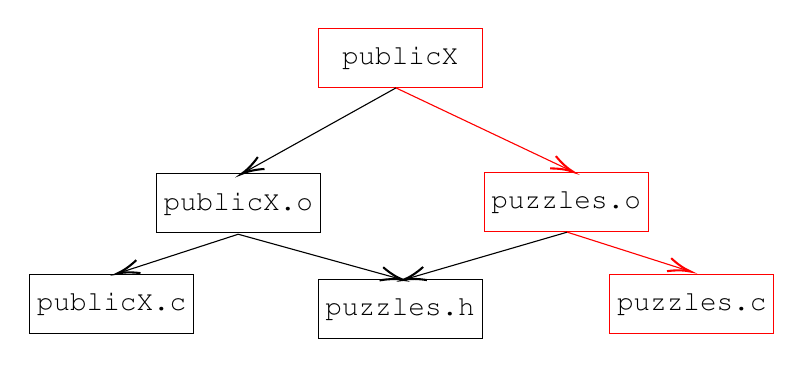
\begin{tikzpicture}[x=0.75pt,y=0.75pt,yscale=-1,xscale=1]
%uncomment if require: \path (0,300); %set diagram left start at 0, and has height of 300

%Shape: Rectangle [id:dp04584351351591953] 
\draw  [color={rgb, 255:red, 255; green, 0; blue, 0 }  ,draw opacity=1 ] (300.5,51) -- (379.5,51) -- (379.5,79.5) -- (300.5,79.5) -- cycle ;
%Shape: Rectangle [id:dp869537413731065] 
\draw  [color={rgb, 255:red, 0; green, 0; blue, 0 }  ,draw opacity=1 ] (222.5,121) -- (301.5,121) -- (301.5,149.5) -- (222.5,149.5) -- cycle ;
%Shape: Rectangle [id:dp09744507127214364] 
\draw  [color={rgb, 255:red, 255; green, 0; blue, 0 }  ,draw opacity=1 ] (380.5,120.5) -- (459.5,120.5) -- (459.5,149) -- (380.5,149) -- cycle ;
%Shape: Rectangle [id:dp6441175322103412] 
\draw   (300.5,172) -- (379.5,172) -- (379.5,200.5) -- (300.5,200.5) -- cycle ;
%Shape: Rectangle [id:dp970334445840234] 
\draw  [color={rgb, 255:red, 0; green, 0; blue, 0 }  ,draw opacity=1 ] (161.5,169.5) -- (240.5,169.5) -- (240.5,198) -- (161.5,198) -- cycle ;
%Shape: Rectangle [id:dp4273912861487811] 
\draw  [color={rgb, 255:red, 255; green, 0; blue, 0 }  ,draw opacity=1 ] (441,169.5) -- (520,169.5) -- (520,198) -- (441,198) -- cycle ;
%Straight Lines [id:da5700845683815001] 
\draw [color={rgb, 255:red, 0; green, 0; blue, 0 }  ,draw opacity=1 ]   (338,79.75) -- (265.25,120.28) ;
\draw [shift={(263.5,121.25)}, rotate = 330.88] [color={rgb, 255:red, 0; green, 0; blue, 0 }  ,draw opacity=1 ][line width=0.75]    (10.93,-3.29) .. controls (6.95,-1.4) and (3.31,-0.3) .. (0,0) .. controls (3.31,0.3) and (6.95,1.4) .. (10.93,3.29)   ;
%Straight Lines [id:da1587431355483161] 
\draw [color={rgb, 255:red, 255; green, 0; blue, 0 }  ,draw opacity=1 ]   (338,79.75) -- (421.69,119.39) ;
\draw [shift={(423.5,120.25)}, rotate = 205.35] [color={rgb, 255:red, 255; green, 0; blue, 0 }  ,draw opacity=1 ][line width=0.75]    (10.93,-3.29) .. controls (6.95,-1.4) and (3.31,-0.3) .. (0,0) .. controls (3.31,0.3) and (6.95,1.4) .. (10.93,3.29)   ;
%Straight Lines [id:da7368979653415088] 
\draw [color={rgb, 255:red, 0; green, 0; blue, 0 }  ,draw opacity=1 ]   (262,150.25) -- (205.4,168.63) ;
\draw [shift={(203.5,169.25)}, rotate = 342.01] [color={rgb, 255:red, 0; green, 0; blue, 0 }  ,draw opacity=1 ][line width=0.75]    (10.93,-3.29) .. controls (6.95,-1.4) and (3.31,-0.3) .. (0,0) .. controls (3.31,0.3) and (6.95,1.4) .. (10.93,3.29)   ;
%Straight Lines [id:da015222657466875456] 
\draw    (262,150.25) -- (339.57,171.72) ;
\draw [shift={(341.5,172.25)}, rotate = 195.47] [color={rgb, 255:red, 0; green, 0; blue, 0 }  ][line width=0.75]    (10.93,-3.29) .. controls (6.95,-1.4) and (3.31,-0.3) .. (0,0) .. controls (3.31,0.3) and (6.95,1.4) .. (10.93,3.29)   ;
%Straight Lines [id:da20417970212364012] 
\draw    (420.5,149.25) -- (343.42,171.69) ;
\draw [shift={(341.5,172.25)}, rotate = 343.77] [color={rgb, 255:red, 0; green, 0; blue, 0 }  ][line width=0.75]    (10.93,-3.29) .. controls (6.95,-1.4) and (3.31,-0.3) .. (0,0) .. controls (3.31,0.3) and (6.95,1.4) .. (10.93,3.29)   ;
%Straight Lines [id:da3319626117155393] 
\draw [color={rgb, 255:red, 255; green, 0; blue, 0 }  ,draw opacity=1 ]   (420.5,149.25) -- (478.09,167.64) ;
\draw [shift={(480,168.25)}, rotate = 197.71] [color={rgb, 255:red, 255; green, 0; blue, 0 }  ,draw opacity=1 ][line width=0.75]    (10.93,-3.29) .. controls (6.95,-1.4) and (3.31,-0.3) .. (0,0) .. controls (3.31,0.3) and (6.95,1.4) .. (10.93,3.29)   ;

% Text Node
\draw (340,65.25) node   [align=left] {{\fontfamily{pcr}\selectfont publicX}};
% Text Node
\draw (262,135.25) node   [align=left] {{\fontfamily{pcr}\selectfont publicX.o}};
% Text Node
\draw (420,134.75) node   [align=left] {{\fontfamily{pcr}\selectfont puzzles.o}};
% Text Node
\draw (340,186.25) node   [align=left] {{\fontfamily{pcr}\selectfont puzzles.h}};
% Text Node
\draw (480.5,183.75) node   [align=left] {{\fontfamily{pcr}\selectfont puzzles.c}};
% Text Node
\draw (201,183.75) node   [align=left] {{\fontfamily{pcr}\selectfont publicX.c}};


\end{tikzpicture}\newline

	Now you may notice that the recurring theme here is that \texttt{publicX} is always recompiled. This is fine! It's intentional! It only makes sense that if we're changing some of the source to what's going to end up in our final executable, our executable needs to be recompiled. The real issue that \texttt{make} is solving for us here is that \textbf{not everything on the lower limbs of the dependency tree needs to be recompiled if we change just one or two little source files}.
	
	\item \textbf{What needs to be compiled if \texttt{puzzles.h} is changed?}\newline
	
	Now this is the big one. If you'll notice on the tree, just about all of our object files and executable depend on \texttt{puzzles.h}. Let's confirm this by drawing and highlighting our dependency tree once again.\newline
	
	

\tikzset{every picture/.style={line width=0.75pt}} %set default line width to 0.75pt        

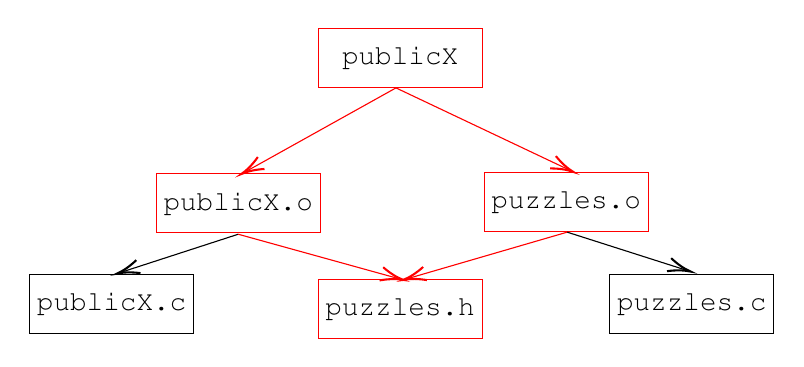
\begin{tikzpicture}[x=0.75pt,y=0.75pt,yscale=-1,xscale=1]
%uncomment if require: \path (0,300); %set diagram left start at 0, and has height of 300

%Shape: Rectangle [id:dp04584351351591953] 
\draw  [color={rgb, 255:red, 255; green, 0; blue, 0 }  ,draw opacity=1 ] (300.5,51) -- (379.5,51) -- (379.5,79.5) -- (300.5,79.5) -- cycle ;
%Shape: Rectangle [id:dp869537413731065] 
\draw  [color={rgb, 255:red, 255; green, 0; blue, 0 }  ,draw opacity=1 ] (222.5,121) -- (301.5,121) -- (301.5,149.5) -- (222.5,149.5) -- cycle ;
%Shape: Rectangle [id:dp09744507127214364] 
\draw  [color={rgb, 255:red, 255; green, 0; blue, 0 }  ,draw opacity=1 ] (380.5,120.5) -- (459.5,120.5) -- (459.5,149) -- (380.5,149) -- cycle ;
%Shape: Rectangle [id:dp6441175322103412] 
\draw  [color={rgb, 255:red, 255; green, 0; blue, 0 }  ,draw opacity=1 ] (300.5,172) -- (379.5,172) -- (379.5,200.5) -- (300.5,200.5) -- cycle ;
%Shape: Rectangle [id:dp970334445840234] 
\draw  [color={rgb, 255:red, 0; green, 0; blue, 0 }  ,draw opacity=1 ] (161.5,169.5) -- (240.5,169.5) -- (240.5,198) -- (161.5,198) -- cycle ;
%Shape: Rectangle [id:dp4273912861487811] 
\draw  [color={rgb, 255:red, 0; green, 0; blue, 0 }  ,draw opacity=1 ] (441,169.5) -- (520,169.5) -- (520,198) -- (441,198) -- cycle ;
%Straight Lines [id:da5700845683815001] 
\draw [color={rgb, 255:red, 255; green, 0; blue, 0 }  ,draw opacity=1 ]   (338,79.75) -- (265.25,120.28) ;
\draw [shift={(263.5,121.25)}, rotate = 330.88] [color={rgb, 255:red, 255; green, 0; blue, 0 }  ,draw opacity=1 ][line width=0.75]    (10.93,-3.29) .. controls (6.95,-1.4) and (3.31,-0.3) .. (0,0) .. controls (3.31,0.3) and (6.95,1.4) .. (10.93,3.29)   ;
%Straight Lines [id:da1587431355483161] 
\draw [color={rgb, 255:red, 255; green, 0; blue, 0 }  ,draw opacity=1 ]   (338,79.75) -- (421.69,119.39) ;
\draw [shift={(423.5,120.25)}, rotate = 205.35] [color={rgb, 255:red, 255; green, 0; blue, 0 }  ,draw opacity=1 ][line width=0.75]    (10.93,-3.29) .. controls (6.95,-1.4) and (3.31,-0.3) .. (0,0) .. controls (3.31,0.3) and (6.95,1.4) .. (10.93,3.29)   ;
%Straight Lines [id:da7368979653415088] 
\draw [color={rgb, 255:red, 0; green, 0; blue, 0 }  ,draw opacity=1 ]   (262,150.25) -- (205.4,168.63) ;
\draw [shift={(203.5,169.25)}, rotate = 342.01] [color={rgb, 255:red, 0; green, 0; blue, 0 }  ,draw opacity=1 ][line width=0.75]    (10.93,-3.29) .. controls (6.95,-1.4) and (3.31,-0.3) .. (0,0) .. controls (3.31,0.3) and (6.95,1.4) .. (10.93,3.29)   ;
%Straight Lines [id:da015222657466875456] 
\draw [color={rgb, 255:red, 255; green, 0; blue, 0 }  ,draw opacity=1 ]   (262,150.25) -- (339.57,171.72) ;
\draw [shift={(341.5,172.25)}, rotate = 195.47] [color={rgb, 255:red, 255; green, 0; blue, 0 }  ,draw opacity=1 ][line width=0.75]    (10.93,-3.29) .. controls (6.95,-1.4) and (3.31,-0.3) .. (0,0) .. controls (3.31,0.3) and (6.95,1.4) .. (10.93,3.29)   ;
%Straight Lines [id:da20417970212364012] 
\draw [color={rgb, 255:red, 255; green, 0; blue, 0 }  ,draw opacity=1 ]   (420.5,149.25) -- (343.42,171.69) ;
\draw [shift={(341.5,172.25)}, rotate = 343.77] [color={rgb, 255:red, 255; green, 0; blue, 0 }  ,draw opacity=1 ][line width=0.75]    (10.93,-3.29) .. controls (6.95,-1.4) and (3.31,-0.3) .. (0,0) .. controls (3.31,0.3) and (6.95,1.4) .. (10.93,3.29)   ;
%Straight Lines [id:da3319626117155393] 
\draw [color={rgb, 255:red, 0; green, 0; blue, 0 }  ,draw opacity=1 ]   (420.5,149.25) -- (478.09,167.64) ;
\draw [shift={(480,168.25)}, rotate = 197.71] [color={rgb, 255:red, 0; green, 0; blue, 0 }  ,draw opacity=1 ][line width=0.75]    (10.93,-3.29) .. controls (6.95,-1.4) and (3.31,-0.3) .. (0,0) .. controls (3.31,0.3) and (6.95,1.4) .. (10.93,3.29)   ;

% Text Node
\draw (340,65.25) node   [align=left] {{\fontfamily{pcr}\selectfont publicX}};
% Text Node
\draw (262,135.25) node   [align=left] {{\fontfamily{pcr}\selectfont publicX.o}};
% Text Node
\draw (420,134.75) node   [align=left] {{\fontfamily{pcr}\selectfont puzzles.o}};
% Text Node
\draw (340,186.25) node   [align=left] {{\fontfamily{pcr}\selectfont puzzles.h}};
% Text Node
\draw (480.5,183.75) node   [align=left] {{\fontfamily{pcr}\selectfont puzzles.c}};
% Text Node
\draw (201,183.75) node   [align=left] {{\fontfamily{pcr}\selectfont publicX.c}};


\end{tikzpicture}\newline

	Even though we didn't change any of the \texttt{.c} files, we changed one of the key nodes in our dependency tree, and for that, we have paid the price. Since both of our object files and ultimately our executable depends on these files, it looks like everything needs to be recompiled after our changes to \texttt{puzzles.h}.


\end{itemize}

So that's how we deal with compilation in makefiles. I invite you to take a look at your old projects that have makefiles in them and change some files around and keep running \texttt{make}. Try drawing your own dependency trees and seeing what recompiles when you make edits to different files. Once you do that enough, you should be ready for any \texttt{make}-related stuff that pops up on an exam.\newline

For more nitty-gritty details on \texttt{make}, definitely take a look at the slides, they have the information you need. However, more or less, exams will probably ask you to either cook up a makefile on your own or decide what will be recompiled if you change some files. I want to make sure that you get the basic concept of all this, so as long as you do what I detail above and remember some of the key points from the slides, you should be in very good shape for exams.\newline

\subsection{Struct Abstraction}

For this section, we'll be talking about Struct Abstraction. For reference, this material can be found at:\newline 

\texttt{216public/labs/Week7/lab2/struct\_abstraction} \newline

I suggest you take a look at the README like we did in discussion, but to get a broad overview of this concept, I want to add a little of my own insight. \newline

Java babied us a lot with its object oriented features and other conveniences, but you'll find that C is a lot less scaffolded. In other words, C does not provide us with the same conveniences that Java does. Struct Abstraction is a fairly niche topic, but it's essentially a reminder to us that we can \textit{sort of} emulate an object oriented feature of Java by naming a struct, yet hiding its implementation. Personally, I haven't found a particular use for it in my 216 projects, but I think it's good knowledge to have. Take a look at the README and work through the example like we did in class, but other than that, make sure you know the gist of it: It's a neat little trick in C that allows us to kind of emulate object oriented behavior by 'hiding' the implementation of a struct.

\subsection{Dynamic Memory Allocation (Review)}

Dynamic memory allocation is one of the most important topics in C, and usually one of the hardest for students to understand. If you haven't fully understood this yet, I would highly suggest either referring back to your lecture notes for the subject, watching older 216 lecture videos on the topic online, or looking at reference material from elsewhere. This will only serve as a quick review + some of my extra insight.\newline

For this section, we'll be looking at the reference material found in the following location:\newline

\texttt{public/labs/Week7/lab2}

\subsubsection{Malloc() vs. Calloc()}

I remember this came up as an exam question during my year, so I think this is an important distinction to remember. When you're looking at allocating memory in C, there are two ways to ask C's memory manager for the space that you need. I like to think of this with the hotel room analogy. When you use \texttt{malloc()}, it's like you've arrived at a hotel and ask the clerk to give you a room (and of course, for the sake of the analogy, let's say you provided a size for the room). Nevermind if it's clean or not, and you don't care what the previous guests left in the room. You just want to know that you have the room, and you'll take care of cleaning it and setting your friends up in it later. \texttt{malloc()} is a function that gives you the memory you're looking for, but it doesn't bother cleaning it out for you- the values at the pointer that \texttt{malloc()} returns can be just about anything- so it's a solid idea not to dereference whatever's there. Now if you use \texttt{calloc()}, that's a different story. That's like asking the clerk for a room, but also adding, "Hey, can you make sure it's cleaned spotless for me?". That way, everything in that room is set to a nice default value and is nice and ready for you to look at- no need to clean it. For example, using \texttt{malloc()} for a string and printing it is a terrible idea, but using \texttt{calloc()} for a string and printing it will work totally fine, as the latter sets the memory to default values.

\subsubsection{Two Pointers to the Same Memory}

C's memory manager isn't smart, but it isn't stupid. If you have two pointers to the same memory that you allocated, using \texttt{free()} to return that chunk of memory to the C memory manager will totally work. Here's an example.\newline

{
\centering


\tikzset{every picture/.style={line width=0.75pt}} %set default line width to 0.75pt        

\begin{tikzpicture}[x=0.75pt,y=0.75pt,yscale=-1,xscale=1]
%uncomment if require: \path (0,300); %set diagram left start at 0, and has height of 300

%Shape: Rectangle [id:dp7660242978805989] 
\draw   (152.5,144.5) -- (222.5,144.5) -- (222.5,184.5) -- (152.5,184.5) -- cycle ;
%Shape: Rectangle [id:dp9835474491940359] 
\draw   (327.5,68) -- (397.5,68) -- (397.5,108) -- (327.5,108) -- cycle ;
%Shape: Rectangle [id:dp6382246899126394] 
\draw   (397.5,68) -- (467.5,68) -- (467.5,108) -- (397.5,108) -- cycle ;
%Shape: Rectangle [id:dp40751687076886434] 
\draw   (467.5,68) -- (537.5,68) -- (537.5,108) -- (467.5,108) -- cycle ;
%Shape: Rectangle [id:dp1956486484356338] 
\draw   (537.5,68) -- (607.5,68) -- (607.5,108) -- (537.5,108) -- cycle ;
%Straight Lines [id:da2803570019045192] 
\draw    (187.5,164.5) -- (326.25,88.21) ;
\draw [shift={(328,87.25)}, rotate = 511.2] [color={rgb, 255:red, 0; green, 0; blue, 0 }  ][line width=0.75]    (10.93,-3.29) .. controls (6.95,-1.4) and (3.31,-0.3) .. (0,0) .. controls (3.31,0.3) and (6.95,1.4) .. (10.93,3.29)   ;

% Text Node
\draw (116,162.5) node   [align=left] {{\fontfamily{pcr}\selectfont ptr\_1}};
% Text Node
\draw (453,49) node   [align=left] {Memory you received from {\fontfamily{pcr}\selectfont malloc()}};


\end{tikzpicture}
}

Here, let's say we used \texttt{malloc()} to grab some memory for \texttt{ptr\_1}. Nevermind what the type of it is, that isn't important.\newline

Now, let's say we set a new pointer \texttt{ptr\_2} equal to \texttt{ptr\_1}. In other words, we now have two pointers pointing to this memory that you've malloc'd.\newline

{
\centering


\tikzset{every picture/.style={line width=0.75pt}} %set default line width to 0.75pt        

\begin{tikzpicture}[x=0.75pt,y=0.75pt,yscale=-1,xscale=1]
%uncomment if require: \path (0,300); %set diagram left start at 0, and has height of 300

%Shape: Rectangle [id:dp7660242978805989] 
\draw   (152.5,144.5) -- (222.5,144.5) -- (222.5,184.5) -- (152.5,184.5) -- cycle ;
%Shape: Rectangle [id:dp9835474491940359] 
\draw   (327.5,68) -- (397.5,68) -- (397.5,108) -- (327.5,108) -- cycle ;
%Shape: Rectangle [id:dp6382246899126394] 
\draw   (397.5,68) -- (467.5,68) -- (467.5,108) -- (397.5,108) -- cycle ;
%Shape: Rectangle [id:dp40751687076886434] 
\draw   (467.5,68) -- (537.5,68) -- (537.5,108) -- (467.5,108) -- cycle ;
%Shape: Rectangle [id:dp1956486484356338] 
\draw   (537.5,68) -- (607.5,68) -- (607.5,108) -- (537.5,108) -- cycle ;
%Straight Lines [id:da2803570019045192] 
\draw    (187.5,164.5) -- (326.25,88.21) ;
\draw [shift={(328,87.25)}, rotate = 511.2] [color={rgb, 255:red, 0; green, 0; blue, 0 }  ][line width=0.75]    (10.93,-3.29) .. controls (6.95,-1.4) and (3.31,-0.3) .. (0,0) .. controls (3.31,0.3) and (6.95,1.4) .. (10.93,3.29)   ;
%Shape: Rectangle [id:dp8693066240275549] 
\draw   (134,22.5) -- (204,22.5) -- (204,62.5) -- (134,62.5) -- cycle ;
%Straight Lines [id:da23910938451416597] 
\draw    (169,42.5) -- (326.07,86.71) ;
\draw [shift={(328,87.25)}, rotate = 195.72] [color={rgb, 255:red, 0; green, 0; blue, 0 }  ][line width=0.75]    (10.93,-3.29) .. controls (6.95,-1.4) and (3.31,-0.3) .. (0,0) .. controls (3.31,0.3) and (6.95,1.4) .. (10.93,3.29)   ;

% Text Node
\draw (116,162.5) node   [align=left] {{\fontfamily{pcr}\selectfont ptr\_1}};
% Text Node
\draw (453,49) node   [align=left] {memory you received from {\fontfamily{pcr}\selectfont malloc()}};
% Text Node
\draw (103,37.5) node   [align=left] {{\fontfamily{pcr}\selectfont ptr\_2}};


\end{tikzpicture}

}

Now, if we want to return this memory back to the memory manager, we can do that very easily by doing either of the following:\newline

\texttt{free(ptr\_2);} or \texttt{free(ptr\_1);}\newline

The reason that this works is that, as far as C is concerned, the actual pointer that you have to the memory that it gave you doesn't matter. At the end of the day, \texttt{free()} takes in a memory address, and C will check to see if it's given you memory at that address. If it decides that it has indeed given you memory at that address, it'll take it back. That's why calling \texttt{free()} on either \texttt{ptr\_1} or \texttt{ptr\_2} will work just fine.

\subsubsection{Malloc with Structs}

One more key point that I want to touch on is that you'll want to use \texttt{sizeof} correctly when allocating memory for structs. When you're allocating memory for a struct, always make sure to allocate memory for the size of the \textbf{struct}, not the size of the \textbf{pointer} to the struct. This is a common mistake, and usually results in segfaults.\newline

\subsubsection{Freeing in the Reverse Order you Malloc}

Here's a good rule of thumb that I like to follow for projects. Whenever you're allocating memory, you'll usually go in a top-down manner. If you have a struct like the one below:\newline

\begin{lstlisting}[language=C]
 typedef struct whale {
   char *name;
   int *weight;
} Whale;
\end{lstlisting}

You'll want to allocate memory for it in order. First, allocate memory for the \texttt{whale} struct itself. Then, remember that the whale struct is only big enough to contain two pointers. If we want those pointers to actually \textbf{point} to anything, we're going to have to allocate that memory too. Thus, we allocate memory for the string \texttt{name} and the int \texttt{weight} as well.\newline

Now, we've got all the memory space we need. Great. But how would we give it back to the program when we're done? Again, follow this rule of thumb: \textbf{free in the reverse order that you malloc}. If you allocated memory for the whale first, then string, then int, go ahead and free the int, the string, then finally the whale. If you don't follow this order and decide to free the whale first, you've effectively lost access to the pointers contained in the whale, and now you won't be able to free that memory. That results in a memory leak, and we definitely don't want that. So again, if you used malloc to allocate memory for \textbf{A}, \textbf{B}, then \textbf{C}, a great rule of thumb is to free \textbf{C}, then \textbf{B}, then finally, \textbf{A}.

Again, these are just a few tips and tricks regarding dynamic memory allocation, but this is an important concept to fully understand in 216. I can't stress the importance of referring to other notes or looking at old lectures until you truly understand dynamic memory allocation.\newline

\subsubsection{Using Valgrind to Find Memory Leaks}

The memory leaks I mentioned above are silent killers- all it takes are a few badly ordered \texttt{free()} function calls, and you've got yourself a memory leak. A great way to check for these quickly is to run \texttt{valgrind}.\newline

It's actually really simple to do so. If you want to check if your executable has any memory leaks, go ahead and use \texttt{make} or \texttt{gcc} to compile it into your executable or an \texttt{a.out} file, then run the following:\newline

\texttt{valgrind a.out} or \texttt{valgrind your\_executable}\newline

If all goes well, \texttt{valgrind} should let you know that 'all blocks were freed'. If not, it will complain and let you know that some pointers were not freed. From there, you can go ahead and examine your code to see where you were making the mistake.\newline

Here's an excellent quick and basic tutorial for using valgrind to check for memory leaks that I used when I was taking 216. If you want further reference, I encourage you to check it out.\newline

\texttt{\href{http://cs.ecs.baylor.edu/~donahoo/tools/valgrind/}{http://cs.ecs.baylor.edu/~donahoo/tools/valgrind/}}

\section{Week 8}

\subsection{Sorting in C}

Sometimes, be it for a project or on an exam, you'll need to quickly sort a list of items (or more specifically, an array of structs). \texttt{qsort()} is basically the quick and easy way to get that done in C. Let's take a look at the actual function definition found on the manpage.\newline

\texttt{void qsort(void *base, size\_t nmemb, size\_t size, int(*compar)(const void *, const void *));}\newline

As all manpage entries are, this may seem confusing at first, so let me break it down for you. \textbf{\texttt{base}} is referring to the array you want to sort in the first place. \textbf{\texttt{nmemb}} is the length of your array, so C knows the bounds of the memory space that it's playing around with. \textbf{\texttt{size}} is the size of the elements in said array, so C knows how big the chunks are that it needs to inevitably move around when it performs the sort. Finally, \textbf{\texttt{compar}} would be your comparator function. This is something I urge you to recall from 132- if you'll recall what a comparator function is, it essentially just tells you if one of the input parameters is 'greater' than the other. If you forgot what a comparator is, another great analog is the \texttt{.compareTo()} method in Java.\newline

There's not much more to it than that. If you ever need your array sorted in C, unless you're explicitly told to write your own algorithm, don't reinvent the wheel. Go ahead and use the \texttt{qsort()} function.

\subsection{The Root User}

On every UNIX system, there is an all-powerful user (superuser) known as \texttt{root}. It's the first user created whenever you install a UNIX machine, and in a weirdly poetic way, all other users are born from it, making it the parent and creator of every other user on a machine.\newline

All you need to know is that it is identified by the name \textbf{root}, it's known as a \textbf{superuser}, and for the purposes of this class, it can basically do anything and everything on the system. In other words, it's the most powerful user on a system.

\subsection{Octal and File Permissions}

Let's talk about file permissions on a UNIX system. Before we do that though, let's do a quick review of the octal number system. You should have the most experience with the decimal system, which uses the digits 0 through 9. Next up, as a CS major, you should be familiar with the binary system, which only uses digits 0 and 1. A key concept to remember is that you can also convert between both, and in that sense, you need to understand that you can represent \textit{any number} in binary or decimal representation, it'll just look different.\newline

That being said, in order to set file permissions on a UNIX system, we take advantage of the \textbf{octal} number system. Just like the latin root \textbf{it} implies, there are 8 total digits that we'll be using, 0 through 7. Now that we understand octal, we can move on to talking about file permissions.\newline

The easiest way to understand something like this is to have hands-on experience. Luckily, we have the grace system at our fingertips to try out stuff like this. Head to your \texttt{216} directory if you'd like to follow along. Go ahead and use \texttt{mkdir} to make a new folder so we can view its permissions. I'm going to name mine 'spaghetti'. If you use the command \texttt{ls -l}, the verbose \texttt{ls} command should show you the file permissions of everything in your current directory (including that of our new directory). Let's focus on what \texttt{ls -l} tells us about the directory for now.\newline

{
\centering


\tikzset{every picture/.style={line width=0.75pt}} %set default line width to 0.75pt        

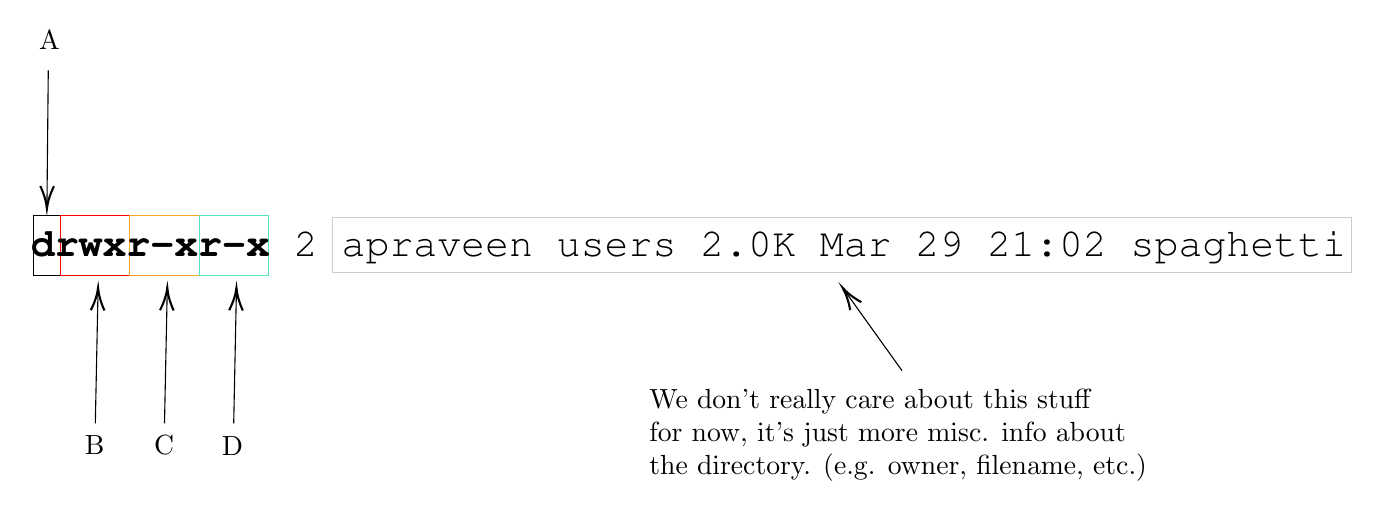
\begin{tikzpicture}[x=0.75pt,y=0.75pt,yscale=-1,xscale=1]
%uncomment if require: \path (0,300); %set diagram left start at 0, and has height of 300

%Shape: Rectangle [id:dp42760139883003023] 
\draw  [color={rgb, 255:red, 205; green, 205; blue, 205 }  ,draw opacity=1 ] (195.33,132.67) -- (686.33,132.67) -- (686.33,159.33) -- (195.33,159.33) -- cycle ;
%Straight Lines [id:da027412161022483783] 
\draw    (469.67,206.67) -- (442.17,168.29) ;
\draw [shift={(441,166.67)}, rotate = 414.37] [color={rgb, 255:red, 0; green, 0; blue, 0 }  ][line width=0.75]    (10.93,-3.29) .. controls (6.95,-1.4) and (3.31,-0.3) .. (0,0) .. controls (3.31,0.3) and (6.95,1.4) .. (10.93,3.29)   ;
%Shape: Rectangle [id:dp36561122366047005] 
\draw   (51,132) -- (64.33,132) -- (64.33,160.67) -- (51,160.67) -- cycle ;
%Straight Lines [id:da43107557729764845] 
\draw    (58.33,62) -- (57.69,126.67) ;
\draw [shift={(57.67,128.67)}, rotate = 270.57] [color={rgb, 255:red, 0; green, 0; blue, 0 }  ][line width=0.75]    (10.93,-3.29) .. controls (6.95,-1.4) and (3.31,-0.3) .. (0,0) .. controls (3.31,0.3) and (6.95,1.4) .. (10.93,3.29)   ;
%Shape: Rectangle [id:dp11069137081996394] 
\draw  [color={rgb, 255:red, 255; green, 0; blue, 0 }  ,draw opacity=1 ] (64.33,132) -- (97.67,132) -- (97.67,160.67) -- (64.33,160.67) -- cycle ;
%Shape: Rectangle [id:dp5105405899279477] 
\draw  [color={rgb, 255:red, 245; green, 166; blue, 35 }  ,draw opacity=1 ] (97.67,132) -- (131,132) -- (131,160.67) -- (97.67,160.67) -- cycle ;
%Shape: Rectangle [id:dp1241998432620336] 
\draw  [color={rgb, 255:red, 80; green, 227; blue, 194 }  ,draw opacity=1 ] (131,132) -- (164.33,132) -- (164.33,160.67) -- (131,160.67) -- cycle ;
%Straight Lines [id:da031602023639908494] 
\draw    (81,232) -- (82.29,168.67) ;
\draw [shift={(82.33,166.67)}, rotate = 451.17] [color={rgb, 255:red, 0; green, 0; blue, 0 }  ][line width=0.75]    (10.93,-3.29) .. controls (6.95,-1.4) and (3.31,-0.3) .. (0,0) .. controls (3.31,0.3) and (6.95,1.4) .. (10.93,3.29)   ;
%Straight Lines [id:da3521048722446102] 
\draw    (114.33,232) -- (115.63,168.67) ;
\draw [shift={(115.67,166.67)}, rotate = 451.17] [color={rgb, 255:red, 0; green, 0; blue, 0 }  ][line width=0.75]    (10.93,-3.29) .. controls (6.95,-1.4) and (3.31,-0.3) .. (0,0) .. controls (3.31,0.3) and (6.95,1.4) .. (10.93,3.29)   ;
%Straight Lines [id:da6073172586106217] 
\draw    (147.67,232) -- (148.96,168.67) ;
\draw [shift={(149,166.67)}, rotate = 451.17] [color={rgb, 255:red, 0; green, 0; blue, 0 }  ][line width=0.75]    (10.93,-3.29) .. controls (6.95,-1.4) and (3.31,-0.3) .. (0,0) .. controls (3.31,0.3) and (6.95,1.4) .. (10.93,3.29)   ;

% Text Node
\draw (48.67,137.67) node [anchor=north west][inner sep=0.75pt]   [align=left] {{\fontfamily{pcr}\selectfont {\Large \textbf{drwxr-xr-x} 2 apraveen users 2.0K Mar 29 21:02 spaghetti}}};
% Text Node
\draw (346.67,214.33) node [anchor=north west][inner sep=0.75pt]   [align=left] {We don't really care about this stuff\\for now, it's just more misc. info about\\the directory. (e.g. owner, filename, etc.)};
% Text Node
\draw (52.67,41.67) node [anchor=north west][inner sep=0.75pt]   [align=left] {A};
% Text Node
\draw (74.67,236.67) node [anchor=north west][inner sep=0.75pt]   [align=left] {B};
% Text Node
\draw (108,236.67) node [anchor=north west][inner sep=0.75pt]   [align=left] {C};
% Text Node
\draw (140.67,237.33) node [anchor=north west][inner sep=0.75pt]   [align=left] {D};


\end{tikzpicture}
}

Let's walk through the diagram that I've made out of the \texttt{ls -l} command above. There isn't any octal in the picture, but I encourage you to keep the idea in your mind for now. First and foremost, let's forget about the grayed out box for now. That's extra stuff that \texttt{ls -l} provides us with, but it won't be that useful when we're talking about file permissions.\newline

\textbf{(A)} represents 'directory'. It's as simple as that- if this entity that we were analyzing using \texttt{ls -l} weren't a directory, we'd simply not see the 'd' there. \textbf{(B)}, the first 3 characters, represent permissions associated with the owner of the file. Since we see a \texttt{r}, \texttt{w}, and an \texttt{x}, we can see that the owner her permissions to \textit{read}, \textit{write}, and \textit{execute} whatever this entity is. In this case, it makes total sense; I made the folder just now, so I should be able to do whatever I want to it. \textbf{(C)}, the second 3 characters, are permissions associated with a group. For now, all you need to remember is that the group that we're referring to is the group to which this particular file/directory belongs. Finally, \textbf{(D)}, the last 3 characters, represent the permissions for everyone. Obviously, we have to be the most careful about these- e.g. if we accidentally give everyone \textit{write} access to all our files, we could have disastrous consequences.\newline

In order to change these set permissions, we can use the \texttt{chmod} command in conjunction with a 3-digit octal parameter, such as \texttt{chmod 700 spaghetti}. Specifically, we would do something like this:\newline

{
\centering


\tikzset{every picture/.style={line width=0.75pt}} %set default line width to 0.75pt        

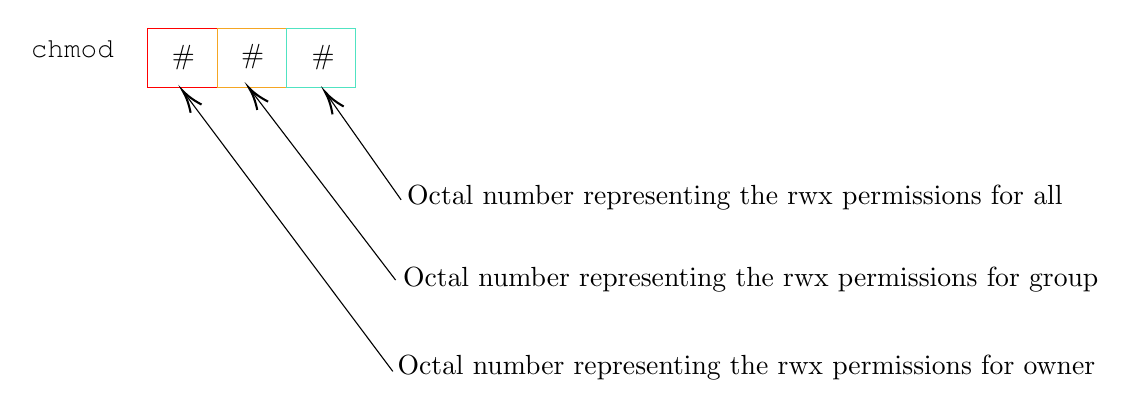
\begin{tikzpicture}[x=0.75pt,y=0.75pt,yscale=-1,xscale=1]
%uncomment if require: \path (0,300); %set diagram left start at 0, and has height of 300

%Shape: Rectangle [id:dp11069137081996394] 
\draw  [color={rgb, 255:red, 255; green, 0; blue, 0 }  ,draw opacity=1 ] (152.33,105.33) -- (185.67,105.33) -- (185.67,134) -- (152.33,134) -- cycle ;
%Shape: Rectangle [id:dp5105405899279477] 
\draw  [color={rgb, 255:red, 245; green, 166; blue, 35 }  ,draw opacity=1 ] (185.67,105.33) -- (219,105.33) -- (219,134) -- (185.67,134) -- cycle ;
%Shape: Rectangle [id:dp1241998432620336] 
\draw  [color={rgb, 255:red, 80; green, 227; blue, 194 }  ,draw opacity=1 ] (219,105.33) -- (252.33,105.33) -- (252.33,134) -- (219,134) -- cycle ;
%Straight Lines [id:da3925814990937547] 
\draw    (270.33,270.67) -- (170.2,136.93) ;
\draw [shift={(169,135.33)}, rotate = 413.18] [color={rgb, 255:red, 0; green, 0; blue, 0 }  ][line width=0.75]    (10.93,-3.29) .. controls (6.95,-1.4) and (3.31,-0.3) .. (0,0) .. controls (3.31,0.3) and (6.95,1.4) .. (10.93,3.29)   ;
%Straight Lines [id:da8411143149408029] 
\draw    (271.67,226.67) -- (202.21,135.59) ;
\draw [shift={(201,134)}, rotate = 412.66999999999996] [color={rgb, 255:red, 0; green, 0; blue, 0 }  ][line width=0.75]    (10.93,-3.29) .. controls (6.95,-1.4) and (3.31,-0.3) .. (0,0) .. controls (3.31,0.3) and (6.95,1.4) .. (10.93,3.29)   ;
%Straight Lines [id:da2927838400275865] 
\draw    (274.33,188) -- (238.82,137.63) ;
\draw [shift={(237.67,136)}, rotate = 414.81] [color={rgb, 255:red, 0; green, 0; blue, 0 }  ][line width=0.75]    (10.93,-3.29) .. controls (6.95,-1.4) and (3.31,-0.3) .. (0,0) .. controls (3.31,0.3) and (6.95,1.4) .. (10.93,3.29)   ;

% Text Node
\draw (162.67,112.33) node [anchor=north west][inner sep=0.75pt]   [align=left] {\#};
% Text Node
\draw (196,111.67) node [anchor=north west][inner sep=0.75pt]   [align=left] {\#};
% Text Node
\draw (230,112.33) node [anchor=north west][inner sep=0.75pt]   [align=left] {\#};
% Text Node
\draw (94.67,109.67) node [anchor=north west][inner sep=0.75pt]   [align=left] {{\fontfamily{pcr}\selectfont chmod}};
% Text Node
\draw (271.33,261.67) node [anchor=north west][inner sep=0.75pt]   [align=left] {Octal number representing the rwx permissions for owner};
% Text Node
\draw (274,219) node [anchor=north west][inner sep=0.75pt]   [align=left] {Octal number representing the rwx permissions for group};
% Text Node
\draw (276,179.67) node [anchor=north west][inner sep=0.75pt]   [align=left] {Octal number representing the rwx permissions for all};


\end{tikzpicture}

}

Think back to when we talked about converting between number systems. Each number in the 3-digit octal parameter that we provide chmod actually represents a configuration for \texttt{rwx}. Specifically, it's that octal number converted to binary. In order to decode what each permission means, we'd convert each digit in the octal input parameter to its binary counterpart, then figure out which permissions were 'active' based on the presence of a 0 or a 1. For example, let's say we wanted to give our file read/write/execute access for everyone. We would execute \texttt{chmod 777 spaghetti}. Below is a diagram explaining the details.\newline

{
\centering


\tikzset{every picture/.style={line width=0.75pt}} %set default line width to 0.75pt        

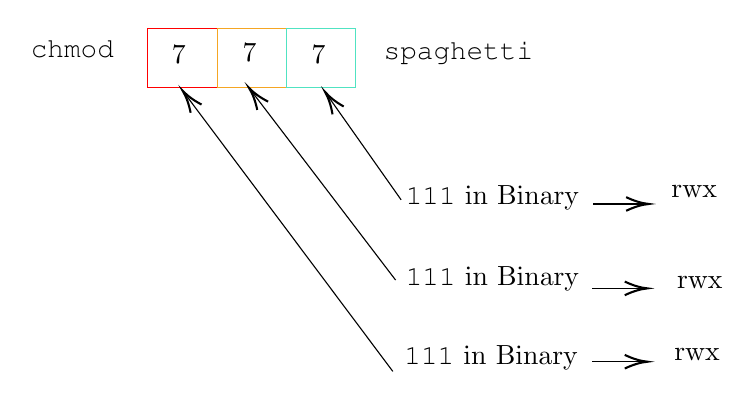
\begin{tikzpicture}[x=0.75pt,y=0.75pt,yscale=-1,xscale=1]
%uncomment if require: \path (0,300); %set diagram left start at 0, and has height of 300

%Shape: Rectangle [id:dp11069137081996394] 
\draw  [color={rgb, 255:red, 255; green, 0; blue, 0 }  ,draw opacity=1 ] (152.33,105.33) -- (185.67,105.33) -- (185.67,134) -- (152.33,134) -- cycle ;
%Shape: Rectangle [id:dp5105405899279477] 
\draw  [color={rgb, 255:red, 245; green, 166; blue, 35 }  ,draw opacity=1 ] (185.67,105.33) -- (219,105.33) -- (219,134) -- (185.67,134) -- cycle ;
%Shape: Rectangle [id:dp1241998432620336] 
\draw  [color={rgb, 255:red, 80; green, 227; blue, 194 }  ,draw opacity=1 ] (219,105.33) -- (252.33,105.33) -- (252.33,134) -- (219,134) -- cycle ;
%Straight Lines [id:da3925814990937547] 
\draw    (270.33,270.67) -- (170.2,136.93) ;
\draw [shift={(169,135.33)}, rotate = 413.18] [color={rgb, 255:red, 0; green, 0; blue, 0 }  ][line width=0.75]    (10.93,-3.29) .. controls (6.95,-1.4) and (3.31,-0.3) .. (0,0) .. controls (3.31,0.3) and (6.95,1.4) .. (10.93,3.29)   ;
%Straight Lines [id:da8411143149408029] 
\draw    (271.67,226.67) -- (202.21,135.59) ;
\draw [shift={(201,134)}, rotate = 412.66999999999996] [color={rgb, 255:red, 0; green, 0; blue, 0 }  ][line width=0.75]    (10.93,-3.29) .. controls (6.95,-1.4) and (3.31,-0.3) .. (0,0) .. controls (3.31,0.3) and (6.95,1.4) .. (10.93,3.29)   ;
%Straight Lines [id:da2927838400275865] 
\draw    (274.33,188) -- (238.82,137.63) ;
\draw [shift={(237.67,136)}, rotate = 414.81] [color={rgb, 255:red, 0; green, 0; blue, 0 }  ][line width=0.75]    (10.93,-3.29) .. controls (6.95,-1.4) and (3.31,-0.3) .. (0,0) .. controls (3.31,0.3) and (6.95,1.4) .. (10.93,3.29)   ;
%Straight Lines [id:da8093183970331216] 
\draw    (367,190) -- (391.67,190) ;
\draw [shift={(393.67,190)}, rotate = 180] [color={rgb, 255:red, 0; green, 0; blue, 0 }  ][line width=0.75]    (10.93,-3.29) .. controls (6.95,-1.4) and (3.31,-0.3) .. (0,0) .. controls (3.31,0.3) and (6.95,1.4) .. (10.93,3.29)   ;
%Straight Lines [id:da9695792273639827] 
\draw    (366.33,230.67) -- (391,230.67) ;
\draw [shift={(393,230.67)}, rotate = 180] [color={rgb, 255:red, 0; green, 0; blue, 0 }  ][line width=0.75]    (10.93,-3.29) .. controls (6.95,-1.4) and (3.31,-0.3) .. (0,0) .. controls (3.31,0.3) and (6.95,1.4) .. (10.93,3.29)   ;
%Straight Lines [id:da1626297191907251] 
\draw    (366.33,266) -- (391,266) ;
\draw [shift={(393,266)}, rotate = 180] [color={rgb, 255:red, 0; green, 0; blue, 0 }  ][line width=0.75]    (10.93,-3.29) .. controls (6.95,-1.4) and (3.31,-0.3) .. (0,0) .. controls (3.31,0.3) and (6.95,1.4) .. (10.93,3.29)   ;

% Text Node
\draw (162.67,112.33) node [anchor=north west][inner sep=0.75pt]   [align=left] {7};
% Text Node
\draw (196.67,111.67) node [anchor=north west][inner sep=0.75pt]   [align=left] {7};
% Text Node
\draw (230,112.33) node [anchor=north west][inner sep=0.75pt]   [align=left] {7};
% Text Node
\draw (94.67,109.67) node [anchor=north west][inner sep=0.75pt]   [align=left] {{\fontfamily{pcr}\selectfont chmod}};
% Text Node
\draw (275.33,179.67) node [anchor=north west][inner sep=0.75pt]   [align=left] {{\fontfamily{pcr}\selectfont 111} in Binary};
% Text Node
\draw (275.33,219) node [anchor=north west][inner sep=0.75pt]   [align=left] {{\fontfamily{pcr}\selectfont 111} in Binary};
% Text Node
\draw (274.67,257) node [anchor=north west][inner sep=0.75pt]   [align=left] {{\fontfamily{pcr}\selectfont 111} in Binary};
% Text Node
\draw (403.33,179.67) node [anchor=north west][inner sep=0.75pt]   [align=left] {rwx};
% Text Node
\draw (406,223.67) node [anchor=north west][inner sep=0.75pt]   [align=left] {rwx};
% Text Node
\draw (404.67,258.33) node [anchor=north west][inner sep=0.75pt]   [align=left] {rwx};
% Text Node
\draw (264.67,110.33) node [anchor=north west][inner sep=0.75pt]   [align=left] {{\fontfamily{pcr}\selectfont spaghetti}};


\end{tikzpicture}


}

Like I explained above, you'll notice that we're taking two basic steps. \newline

\begin{itemize}
	\item \texttt{First}, convert each octal input digit to binary.
	\item \texttt{Second}, see where the ones and zeroes are in that binary output, and that'll tell you which of the rwx parameters are active.
\end{itemize}

For example, if you wanted rwx permissions for everyone like we set above, except this time, we'd only allow all users outside of the owner and the file group to only read the file, we'd edit the last digit in the octal input parameter to reflect that, like so:\newline


{
\centering


\tikzset{every picture/.style={line width=0.75pt}} %set default line width to 0.75pt        

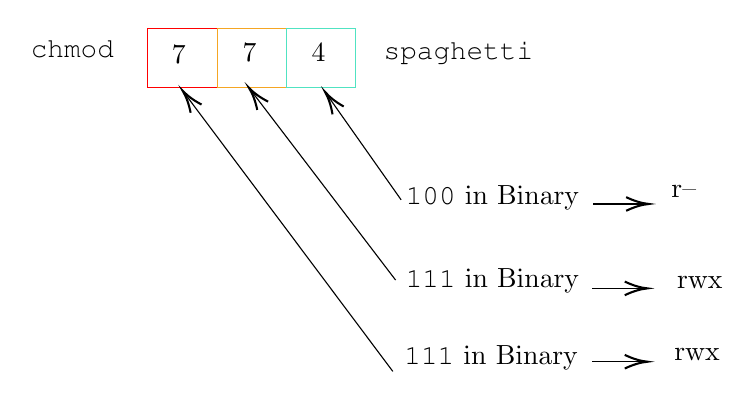
\begin{tikzpicture}[x=0.75pt,y=0.75pt,yscale=-1,xscale=1]
%uncomment if require: \path (0,300); %set diagram left start at 0, and has height of 300

%Shape: Rectangle [id:dp11069137081996394] 
\draw  [color={rgb, 255:red, 255; green, 0; blue, 0 }  ,draw opacity=1 ] (152.33,105.33) -- (185.67,105.33) -- (185.67,134) -- (152.33,134) -- cycle ;
%Shape: Rectangle [id:dp5105405899279477] 
\draw  [color={rgb, 255:red, 245; green, 166; blue, 35 }  ,draw opacity=1 ] (185.67,105.33) -- (219,105.33) -- (219,134) -- (185.67,134) -- cycle ;
%Shape: Rectangle [id:dp1241998432620336] 
\draw  [color={rgb, 255:red, 80; green, 227; blue, 194 }  ,draw opacity=1 ] (219,105.33) -- (252.33,105.33) -- (252.33,134) -- (219,134) -- cycle ;
%Straight Lines [id:da3925814990937547] 
\draw    (270.33,270.67) -- (170.2,136.93) ;
\draw [shift={(169,135.33)}, rotate = 413.18] [color={rgb, 255:red, 0; green, 0; blue, 0 }  ][line width=0.75]    (10.93,-3.29) .. controls (6.95,-1.4) and (3.31,-0.3) .. (0,0) .. controls (3.31,0.3) and (6.95,1.4) .. (10.93,3.29)   ;
%Straight Lines [id:da8411143149408029] 
\draw    (271.67,226.67) -- (202.21,135.59) ;
\draw [shift={(201,134)}, rotate = 412.66999999999996] [color={rgb, 255:red, 0; green, 0; blue, 0 }  ][line width=0.75]    (10.93,-3.29) .. controls (6.95,-1.4) and (3.31,-0.3) .. (0,0) .. controls (3.31,0.3) and (6.95,1.4) .. (10.93,3.29)   ;
%Straight Lines [id:da2927838400275865] 
\draw    (274.33,188) -- (238.82,137.63) ;
\draw [shift={(237.67,136)}, rotate = 414.81] [color={rgb, 255:red, 0; green, 0; blue, 0 }  ][line width=0.75]    (10.93,-3.29) .. controls (6.95,-1.4) and (3.31,-0.3) .. (0,0) .. controls (3.31,0.3) and (6.95,1.4) .. (10.93,3.29)   ;
%Straight Lines [id:da8093183970331216] 
\draw    (367,190) -- (391.67,190) ;
\draw [shift={(393.67,190)}, rotate = 180] [color={rgb, 255:red, 0; green, 0; blue, 0 }  ][line width=0.75]    (10.93,-3.29) .. controls (6.95,-1.4) and (3.31,-0.3) .. (0,0) .. controls (3.31,0.3) and (6.95,1.4) .. (10.93,3.29)   ;
%Straight Lines [id:da9695792273639827] 
\draw    (366.33,230.67) -- (391,230.67) ;
\draw [shift={(393,230.67)}, rotate = 180] [color={rgb, 255:red, 0; green, 0; blue, 0 }  ][line width=0.75]    (10.93,-3.29) .. controls (6.95,-1.4) and (3.31,-0.3) .. (0,0) .. controls (3.31,0.3) and (6.95,1.4) .. (10.93,3.29)   ;
%Straight Lines [id:da1626297191907251] 
\draw    (366.33,266) -- (391,266) ;
\draw [shift={(393,266)}, rotate = 180] [color={rgb, 255:red, 0; green, 0; blue, 0 }  ][line width=0.75]    (10.93,-3.29) .. controls (6.95,-1.4) and (3.31,-0.3) .. (0,0) .. controls (3.31,0.3) and (6.95,1.4) .. (10.93,3.29)   ;

% Text Node
\draw (162.67,112.33) node [anchor=north west][inner sep=0.75pt]   [align=left] {7};
% Text Node
\draw (196.67,111.67) node [anchor=north west][inner sep=0.75pt]   [align=left] {7};
% Text Node
\draw (230,111.67) node [anchor=north west][inner sep=0.75pt]   [align=left] {4};
% Text Node
\draw (94.67,109.67) node [anchor=north west][inner sep=0.75pt]   [align=left] {{\fontfamily{pcr}\selectfont chmod}};
% Text Node
\draw (275.33,179.67) node [anchor=north west][inner sep=0.75pt]   [align=left] {{\fontfamily{pcr}\selectfont 100} in Binary};
% Text Node
\draw (275.33,219.67) node [anchor=north west][inner sep=0.75pt]   [align=left] {{\fontfamily{pcr}\selectfont 111} in Binary};
% Text Node
\draw (274.67,257) node [anchor=north west][inner sep=0.75pt]   [align=left] {{\fontfamily{pcr}\selectfont 111} in Binary};
% Text Node
\draw (403.33,179.67) node [anchor=north west][inner sep=0.75pt]   [align=left] {r--};
% Text Node
\draw (406,223.67) node [anchor=north west][inner sep=0.75pt]   [align=left] {rwx};
% Text Node
\draw (404.67,258.33) node [anchor=north west][inner sep=0.75pt]   [align=left] {rwx};
% Text Node
\draw (264.67,110.33) node [anchor=north west][inner sep=0.75pt]   [align=left] {{\fontfamily{pcr}\selectfont spaghetti}};


\end{tikzpicture}

}

This is a great way to see the intuitive conversion we have from octal digit to binary to rwx permission. Just remember the two steps I've listed above, and make sure you understand this example, and you should be set. Here are a few more commonly used \texttt{chmod} commands that you may see in the future. In order to fully understand this, I highly recommend you take the examples I'm listing below and work through diagrams like the one I've made above for each of them. If you do that, you'll be in great shape for the exam, where this is fairly likely to show up. (It was on my exam when I took this class).\newline

For these examples, assume again that we have a file named \textbf{spaghetti} that we'd like to change the permissions of. \newline

\begin{itemize}
	\item \texttt{chmod 700 spaghetti} $\rightarrow$ Read write and execute permission for owner, with no access to anyone else (remember, 0 is like --- in rwx notation).
	\item \texttt{chmod 500 spaghetti} $\rightarrow$ Read and execute permissions for owner with no access to anyone else.
	\item \texttt{chmod 755 spaghetti} $\rightarrow$ Read, write, and execute permission for the owner, and read and execute for the group and the rest of the users. If you'll look on grace, you'll see that this is frequently employed by our instructors when they post new material.
\end{itemize}

As a little closing note, you can use \texttt{chmod -R} to recursively change file permissions in the same way that you'd use \texttt{cp -r} to perform a recursive copy. This comes in handy if you're trying to change the permissions of everything within a directory, including subdirectories.





\section{Closing Thoughts}

This document will be updated frequently as we progress through CMSC216. Please send errors to \texttt{apraveen@cs.umd.edu}\newline

\textbf{New as of Mar. 2020: Due to the migration to online classes for the duration of the COVID-19 University Closure, this document will be updated more frequently for the convenience of students.}

\end{document}